% Options for packages loaded elsewhere
\PassOptionsToPackage{unicode}{hyperref}
\PassOptionsToPackage{hyphens}{url}
%
\documentclass[
]{book}
\usepackage{amsmath,amssymb}
\usepackage{lmodern}
\usepackage{iftex}
\ifPDFTeX
  \usepackage[T1]{fontenc}
  \usepackage[utf8]{inputenc}
  \usepackage{textcomp} % provide euro and other symbols
\else % if luatex or xetex
  \usepackage{unicode-math}
  \defaultfontfeatures{Scale=MatchLowercase}
  \defaultfontfeatures[\rmfamily]{Ligatures=TeX,Scale=1}
\fi
% Use upquote if available, for straight quotes in verbatim environments
\IfFileExists{upquote.sty}{\usepackage{upquote}}{}
\IfFileExists{microtype.sty}{% use microtype if available
  \usepackage[]{microtype}
  \UseMicrotypeSet[protrusion]{basicmath} % disable protrusion for tt fonts
}{}
\makeatletter
\@ifundefined{KOMAClassName}{% if non-KOMA class
  \IfFileExists{parskip.sty}{%
    \usepackage{parskip}
  }{% else
    \setlength{\parindent}{0pt}
    \setlength{\parskip}{6pt plus 2pt minus 1pt}}
}{% if KOMA class
  \KOMAoptions{parskip=half}}
\makeatother
\usepackage{xcolor}
\IfFileExists{xurl.sty}{\usepackage{xurl}}{} % add URL line breaks if available
\IfFileExists{bookmark.sty}{\usepackage{bookmark}}{\usepackage{hyperref}}
\hypersetup{
  pdftitle={New York Bight Ecological Model (NYBEM)},
  pdfauthor={S. Kyle McKay, Vanessa Mahan, Michael Dougherty, Toddd Swannack, Candice Hall, Christina Saltus, Molly Reif, Steve Allen},
  hidelinks,
  pdfcreator={LaTeX via pandoc}}
\urlstyle{same} % disable monospaced font for URLs
\usepackage{color}
\usepackage{fancyvrb}
\newcommand{\VerbBar}{|}
\newcommand{\VERB}{\Verb[commandchars=\\\{\}]}
\DefineVerbatimEnvironment{Highlighting}{Verbatim}{commandchars=\\\{\}}
% Add ',fontsize=\small' for more characters per line
\usepackage{framed}
\definecolor{shadecolor}{RGB}{248,248,248}
\newenvironment{Shaded}{\begin{snugshade}}{\end{snugshade}}
\newcommand{\AlertTok}[1]{\textcolor[rgb]{0.94,0.16,0.16}{#1}}
\newcommand{\AnnotationTok}[1]{\textcolor[rgb]{0.56,0.35,0.01}{\textbf{\textit{#1}}}}
\newcommand{\AttributeTok}[1]{\textcolor[rgb]{0.77,0.63,0.00}{#1}}
\newcommand{\BaseNTok}[1]{\textcolor[rgb]{0.00,0.00,0.81}{#1}}
\newcommand{\BuiltInTok}[1]{#1}
\newcommand{\CharTok}[1]{\textcolor[rgb]{0.31,0.60,0.02}{#1}}
\newcommand{\CommentTok}[1]{\textcolor[rgb]{0.56,0.35,0.01}{\textit{#1}}}
\newcommand{\CommentVarTok}[1]{\textcolor[rgb]{0.56,0.35,0.01}{\textbf{\textit{#1}}}}
\newcommand{\ConstantTok}[1]{\textcolor[rgb]{0.00,0.00,0.00}{#1}}
\newcommand{\ControlFlowTok}[1]{\textcolor[rgb]{0.13,0.29,0.53}{\textbf{#1}}}
\newcommand{\DataTypeTok}[1]{\textcolor[rgb]{0.13,0.29,0.53}{#1}}
\newcommand{\DecValTok}[1]{\textcolor[rgb]{0.00,0.00,0.81}{#1}}
\newcommand{\DocumentationTok}[1]{\textcolor[rgb]{0.56,0.35,0.01}{\textbf{\textit{#1}}}}
\newcommand{\ErrorTok}[1]{\textcolor[rgb]{0.64,0.00,0.00}{\textbf{#1}}}
\newcommand{\ExtensionTok}[1]{#1}
\newcommand{\FloatTok}[1]{\textcolor[rgb]{0.00,0.00,0.81}{#1}}
\newcommand{\FunctionTok}[1]{\textcolor[rgb]{0.00,0.00,0.00}{#1}}
\newcommand{\ImportTok}[1]{#1}
\newcommand{\InformationTok}[1]{\textcolor[rgb]{0.56,0.35,0.01}{\textbf{\textit{#1}}}}
\newcommand{\KeywordTok}[1]{\textcolor[rgb]{0.13,0.29,0.53}{\textbf{#1}}}
\newcommand{\NormalTok}[1]{#1}
\newcommand{\OperatorTok}[1]{\textcolor[rgb]{0.81,0.36,0.00}{\textbf{#1}}}
\newcommand{\OtherTok}[1]{\textcolor[rgb]{0.56,0.35,0.01}{#1}}
\newcommand{\PreprocessorTok}[1]{\textcolor[rgb]{0.56,0.35,0.01}{\textit{#1}}}
\newcommand{\RegionMarkerTok}[1]{#1}
\newcommand{\SpecialCharTok}[1]{\textcolor[rgb]{0.00,0.00,0.00}{#1}}
\newcommand{\SpecialStringTok}[1]{\textcolor[rgb]{0.31,0.60,0.02}{#1}}
\newcommand{\StringTok}[1]{\textcolor[rgb]{0.31,0.60,0.02}{#1}}
\newcommand{\VariableTok}[1]{\textcolor[rgb]{0.00,0.00,0.00}{#1}}
\newcommand{\VerbatimStringTok}[1]{\textcolor[rgb]{0.31,0.60,0.02}{#1}}
\newcommand{\WarningTok}[1]{\textcolor[rgb]{0.56,0.35,0.01}{\textbf{\textit{#1}}}}
\usepackage{longtable,booktabs,array}
\usepackage{calc} % for calculating minipage widths
% Correct order of tables after \paragraph or \subparagraph
\usepackage{etoolbox}
\makeatletter
\patchcmd\longtable{\par}{\if@noskipsec\mbox{}\fi\par}{}{}
\makeatother
% Allow footnotes in longtable head/foot
\IfFileExists{footnotehyper.sty}{\usepackage{footnotehyper}}{\usepackage{footnote}}
\makesavenoteenv{longtable}
\usepackage{graphicx}
\makeatletter
\def\maxwidth{\ifdim\Gin@nat@width>\linewidth\linewidth\else\Gin@nat@width\fi}
\def\maxheight{\ifdim\Gin@nat@height>\textheight\textheight\else\Gin@nat@height\fi}
\makeatother
% Scale images if necessary, so that they will not overflow the page
% margins by default, and it is still possible to overwrite the defaults
% using explicit options in \includegraphics[width, height, ...]{}
\setkeys{Gin}{width=\maxwidth,height=\maxheight,keepaspectratio}
% Set default figure placement to htbp
\makeatletter
\def\fps@figure{htbp}
\makeatother
\setlength{\emergencystretch}{3em} % prevent overfull lines
\providecommand{\tightlist}{%
  \setlength{\itemsep}{0pt}\setlength{\parskip}{0pt}}
\setcounter{secnumdepth}{5}
\usepackage{booktabs}
\usepackage{booktabs}
\usepackage{longtable}
\usepackage{array}
\usepackage{multirow}
\usepackage{wrapfig}
\usepackage{float}
\usepackage{colortbl}
\usepackage{pdflscape}
\usepackage{tabu}
\usepackage{threeparttable}
\usepackage{threeparttablex}
\usepackage[normalem]{ulem}
\usepackage{makecell}
\usepackage{xcolor}
\ifLuaTeX
  \usepackage{selnolig}  % disable illegal ligatures
\fi
\usepackage[]{natbib}
\bibliographystyle{apalike}

\title{New York Bight Ecological Model (NYBEM)}
\author{S. Kyle McKay, Vanessa Mahan, Michael Dougherty, Toddd Swannack, Candice Hall, Christina Saltus, Molly Reif, Steve Allen}
\date{2022-03-15}

\begin{document}
\maketitle

{
\setcounter{tocdepth}{1}
\tableofcontents
}
\hypertarget{front-matter}{%
\chapter*{Front Matter}\label{front-matter}}
\addcontentsline{toc}{chapter}{Front Matter}

\hypertarget{point-of-contact}{%
\section*{Point of Contact}\label{point-of-contact}}
\addcontentsline{toc}{section}{Point of Contact}

S. Kyle McKay, Ph.D., P.E.\\
kyle.mckay at usace.army.mil\\
Phone: 970-980-9747\\
Environmental Laboratory\\
New York, NY 10278

{AUTHOR NOTE: All chapters or sections marked with an (I) are incomplete and sections marked with an (i) require minor edits!}

\hypertarget{abstract}{%
\section*{Abstract}\label{abstract}}
\addcontentsline{toc}{section}{Abstract}

The U.S. Army Corps of Engineers (USACE) is conducting three large-scale coastal storm risk management feasibility studies in the New York Bight ecosystem, specifically: the New Jersey Back Bays, the New York-New Jersey Harbor \& Tributaries Study, and the Nassau County Back Bays. In these study areas, the USACE is considering a diversity of measures for mitigating flood risks, including: structural actions (e.g., levees, floodwalls, storm surge barriers), non-structural measures (e.g., buy-outs, elevation of structures, flood-proofing), and natural and nature-based features (e.g., wetland creation, reefs for breakwaters). Environmental outcomes and acceptability are important constraints on plan selection, and the studies are applying a ``tiered'' approach to compliance with the National Environmental Policy Act. The New York Bight Ecological Model (NYBEM) is being developed as a tool for partially assessing the direct and indirect effects of agency actions on regional ecosystems. The NYBEM currently assesses changes in habitat quantity associated with changing hydrodynamics, although future versions will include assessment of habitat quality and changes in aquatic connectivity. This report documents ecological model development processes to date, including information on model scoping, the development process, conceptualization, quantification, and evaluation. The NYBEM is then applied to the New Jersey Back Bays study to assess the extent of potential changes in habitat quantity associated with six alignments of inlet and bay closure structures. The direct, ``footprint'' effects of this infrastructure range from 71 to 182 acres of aquatic ecosystems. The indirect, ``offsite'' effects of this infrastructure lead to habitat switching from estuarine-intertidal and freshwater ecosystems to estuarine-subtidal and upland ecosystems. The magnitude of switching varies based on the six alternative alignments from 418 ac to as much as 938 acres. These estimates do not currently incorporate changes in habitat quality, but instead only account for tidal ranges and salinity thresholds.

\hypertarget{acknowledgements}{%
\section*{Acknowledgements}\label{acknowledgements}}
\addcontentsline{toc}{section}{Acknowledgements}

Model development was funded by the U.S. Army Corps of Engineers through the New Jersey Back Bays (\href{https://www.nap.usace.army.mil/Missions/Civil-Works/New-Jersey-Back-Bays-Coastal-Storm-Risk-Management/}{NJBB}) and NY/NJ Harbor and Tributaries Study (\href{https://www.nan.usace.army.mil/Missions/Civil-Works/Projects-in-New-York/New-York-New-Jersey-Harbor-Tributaries-Focus-Area-Feasibility-Study/}{HATS}). The U.S. Army Corps of Engineers also partially funded research aspects of this work through the Ecosystem Management and Restoration Research Program. The authors are grateful to the USACE project team members and workshop attendees for their generous contributions of time, energy, and ideas. In particular, Bryce Wisemiller and JB Smith managed the larger USACE studies; Rob Hampson, Tate McAlpin, Jennifer McAlpin, and Anthony Emiren coordinated and conducted all hydrodynamic modeling; Cheryl Alkemeyer led environmental impact assessment for the HATS; and Jess Miller provided input and contributions throughout model development. Opinions expressed here are those of the authors and not necessarily those of the agencies they represent.

\hypertarget{glossary-and-acronymns}{%
\section*{Glossary and Acronymns}\label{glossary-and-acronymns}}
\addcontentsline{toc}{section}{Glossary and Acronymns}

\begin{itemize}
\tightlist
\item
  \emph{\href{https://adcirc.org/}{ADCIRC}}: ``a system of computer programs for solving time dependent, free surface circulation and transport problems in two and three dimensions. These programs utilize the finite element method in space allowing the use of highly flexible, unstructured grids.'' For this study, ADCIRC was used to predict storm surge.
\item
  \emph{\href{https://www.erdc.usace.army.mil/Media/Fact-Sheets/Fact-Sheet-Article-View/Article/476708/ada/}{AdH}}: Adaptive Hydraulics (AdH) numerical code is ``a modular, parallel, adaptive finite-element model for one-, two- and three-dimensional (2D, and 3D) flow and transport.'' For this study, AdH was used to predict changes in local hydrodynamics.
\item
  \emph{ADM}: USACE Agency Decision Milestone.
\item
  \emph{AMM}: USACE Alternatives Milestone.
\item
  \emph{Deepwater Ecosystems}: Coastal ecosystems with bed elevation between -2m and -20m below Mean Sea Level (MSL).
\item
  \emph{EIS}: Environmental Impact Statement.
\item
  \emph{ERDC}: U.S. Army Engineer Research and Development Center.\\
\item
  \emph{Estuarine Ecosystems}: Coastal ecosystems with salinity from 0.5 to 30 ppt.
\item
  \emph{Freshwater Ecosystems}: Coastal ecosystems with salinity \textless{} 0.5 ppt.
\item
  \emph{FWOP}: Future WithOut Project Conditions.
\item
  \emph{HATS}: New York / New Jersey Harbor and Tributaries storm risk management study led by the USACE New York District.\\
\item
  \emph{Intertidal Ecosystems}: Coastal ecosystems with bed elevation between Mean Higher High Water (MHHW) and Mean Lower Low Water (MLLW).
\item
  \emph{Marine Ecosystems}: Coastal ecosystems with salinity \textgreater= 30 ppt.
\item
  \emph{Mean Higher High Water (MHHW)}: A tidal datum. The average of the higher high water height each tidal day observed over AdH simulation period (\href{https://shoreline.noaa.gov/glossary.html}{NOAA 2019}).
\item
  \emph{Mean Lower Low Water (MLLW)}: A tidal datum. The average of the lower low water height each tidal day observed over AdH simulation period (\href{https://shoreline.noaa.gov/glossary.html}{NOAA 2019}).
\item
  \emph{MSL}: Mean Sea Level.
\item
  \emph{NAB}: U.S. Army Corps of Engineers Baltimore District.\\
\item
  \emph{NAN}: U.S. Army Corps of Engineers New York District.\\
\item
  \emph{NAP}: U.S. Army Corps of Engineers Philadelphia District.\\
\item
  \emph{NEPA}: National Environmental Policy Act.
\item
  \emph{NLCD}: National Land Cover Dataset\\
\item
  \emph{NCBB}: Nassau County Back Bays coastal storm risk management study led by the USACE Philadelphia District.\\
\item
  \emph{NJBB}: New Jersey Back Bays coastal storm risk management study led by the USACE Philadelphia District.\\
\item
  \emph{NYBEM}: New York Bight Ecological Model (``nigh-bem'').\\
\item
  \emph{PED}: Pre-construction Engineering and Design.
\item
  \emph{Subtidal Ecosystems}: Coastal ecosystems with bed elevation between Mean Lower Low Water (MLLW) and -2m below Mean Sea Level (MSL).
\item
  \emph{TSP}: Tentatively Selected Plan.
\item
  \emph{USACE}: U.S. Army Corps of Engineers.\\
\item
  \emph{USFWS}: U.S. Fish and Wildlife Service.
\end{itemize}

\hypertarget{background}{%
\chapter{Background}\label{background}}

In response to Superstorm Sandy and associated Congressional directives (\href{https://www.congress.gov/113/plaws/publ2/PLAW-113publ2.pdf}{PL 113-2}), the North Atlantic Coast Comprehensive Study (\href{https://www.nad.usace.army.mil/CompStudy/}{NACCS}) identified nine focus areas with populations vulnerable to coastal flooding risk. Three of these areas are in the New York Bight ecosystem, and the U.S. Army Corps of Engineers (USACE) is conducting three large-scale coastal storm risk management (CSRM) feasibility studies. The New Jersey Back Bays (\href{https://www.nap.usace.army.mil/Missions/Civil-Works/New-Jersey-Back-Bays-Coastal-Storm-Risk-Management/}{NJBB}) study is investigating 900 mi\textsuperscript{2} of land and water areas along with 3,400 mi of shoreline spanning a significant portion of New Jersey's Atlantic coastline. The New York-New Jersey Harbor \& Tributaries Study (\href{https://www.nan.usace.army.mil/Missions/Civil-Works/Projects-in-New-York/New-York-New-Jersey-Harbor-Tributaries-Focus-Area-Feasibility-Study/}{HATS}) is examining 2,100 mi\textsuperscript{2} and comprises parts of 25 counties in the two states. The Nassau County Back Bays (\href{https://www.nap.usace.army.mil/Missions/Civil-Works/Nassau-County-Back-Bays-Study/}{NCBB}) study is investigating flood risk in 400 mi\textsuperscript{2} of land and water areas on Long Island's southern shore. Objectives of these studies include issues such as: (a) reduction of coastal storm damage risks to communities, public infrastructure, important societal resources, and the environment, (b) improvement of a community's ability to recover from storm surge damages, (c) enhancement of human health and safety by improving performance of critical infrastructure and natural features during and after storm surge events, and (d) enhancement of coastal resilience with nature-based features.

\begin{figure}
\centering
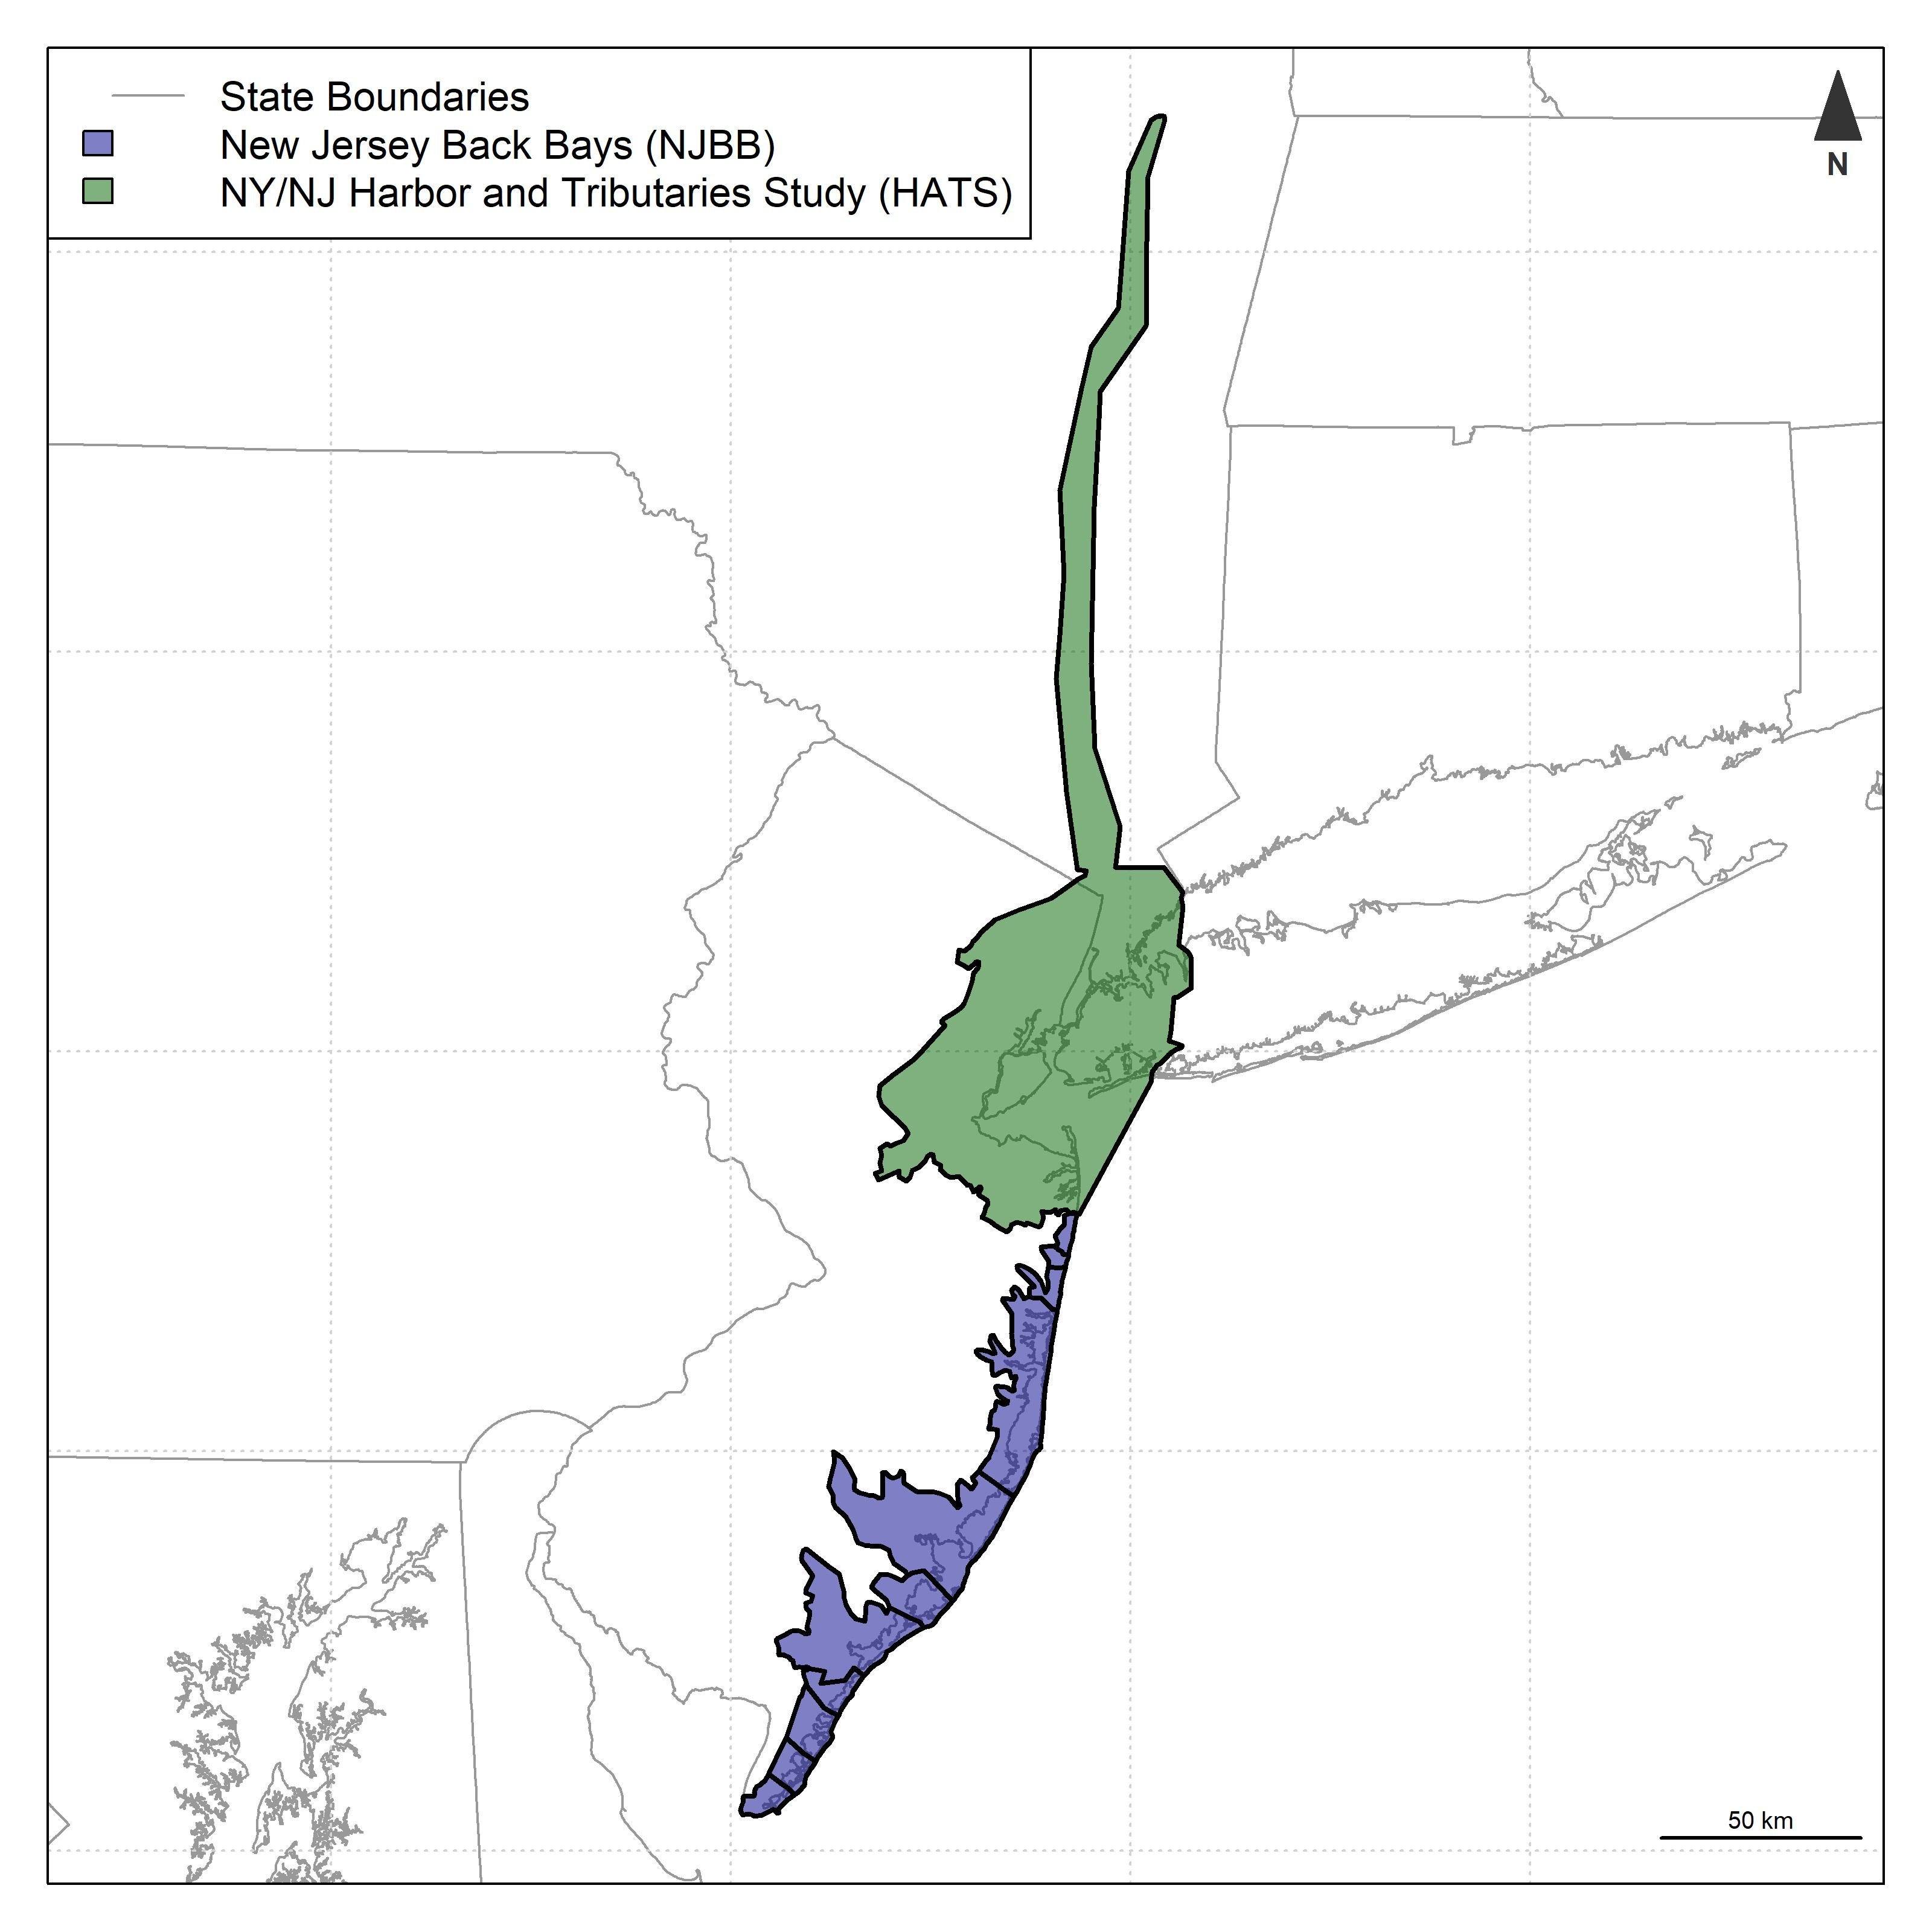
\includegraphics{ZZ_Fig01_USACE.Studies.jpeg}
\caption{\emph{Figure 1. USACE regional coastal storm risk management studies. NJBB and HATS are the primary focus of model development.}}
\end{figure}

In these study areas, the USACE is considering a diversity of measures for mitigating flood risks, including: structural actions (e.g., levees, floodwalls, storm surge barriers), non-structural measures (e.g., buy-outs, elevation of structures, flood-proofing), and natural and nature-based features (NNBF, e.g., wetland creation, reefs for breakwaters). Environmental outcomes and acceptability are important constraints on plan selection, and recommended plans must be in compliance with environmental laws and regulations. Given the large spatial scope, these USACE studies are applying a ``tiered'' approach to compliance with the National Environmental Policy Act (NEPA). Tiered assessment intends to provide appropriate data at key planning milestones for complex studies with diverse environmental effects. In the context of these studies, a ``Tier 1'' Environmental Impact Statement (EIS) will be generated at the conclusion of the USACE Planning Process (i.e., in the Feasibility Report and Chief's Report). A ``Tier 2'' EIS will be developed in Pre-Construction Engineering and Design (PED). The ``Tier 1'' EIS is being developed with sequentially more accurate and precise information as the planning process proceed through key milestones such as the Alternatives Milestone Meeting (AMM), Tentatively Selected Plan Milestone (TSP), and Agency Decision Milestone (ADM).

\hypertarget{problem-statement}{%
\section{Problem Statement}\label{problem-statement}}

The conceptual and numerical models presented here seek to articulate and quantify mechanisms of environmental impact of proposed coastal storm risk management alternatives. The following goals guided model development:

\begin{itemize}
\item
  Models should provide a general description of the \emph{relative} environmental effects of large-scale alternatives, which can inform the feasibility process and NEPA assessments.
\item
  Models must be able to forecast environmental effects over the project planning horizon (50-100 years) based on physical changes to ecosystems resulting from both background processes (e.g., sea level rise) and project alternatives (e.g., change in tidal regime from storm surge barriers).
\item
  Models should assess environmental effects by ecosystem type (e.g., marine deepwater vs.~estuarine intertidal) to inform mitigation actions.
\item
  Models should capture direct effects of actions at infrastructure locations (e.g., the footprint of a floodwall) as well as indirect effects induced off-site from infrastructure (e.g., change in back bay hydrodynamics associated with a storm surge barrier).
\item
  Models should be adaptable to new information and data as project planning proceeds.
\item
  Models should provide a consistent approach for environmental assessment, which can assist with communication of cumulative effects of recommended alternatives across the region.
\end{itemize}

\hypertarget{report-overview}{%
\section{Report Overview}\label{report-overview}}

This report presents development and application of the New York Bight Ecological Model (NYBEM, ``nigh-bem''), which will ultimately consist of two primary sub-models. First, an index-based modeling framework (i.e., a habitat-suitability-style, quantity-quality approach) is applied to assess patch-scale effects for six ecosystem types (e.g., estuarine intertidal zones). Second, a network-based model will be used to assess system-wide connectivity for migratory, aquatic organisms (e.g., anadramous fish). This report provides documentation of the technical details, use, and relevant information for USACE model certification (EC 1105-2-412, PB 2013-02). The following sections summarize the major elements of model development:

\begin{itemize}
\item
  \emph{Model Development Process}: Summarizes the general approach for modeling and the scope of the model.
\item
  \emph{Conceptualization}: Describes the overarching view of the structure and function of ecosystems in the New York Bight.
\item
  \emph{Quantification}: Reviews the technical details of the models.
\item
  \emph{Evaluation}: Assesses the models relative to underlying numerical accuracy, scientific theory, and usability.
\item
  \emph{Application and Communication}: Describes application of models and communication of outcomes for the existing condition in the New Jersey Back Bays (NJBB).
\end{itemize}

\hypertarget{model-development-process}{%
\chapter{Model Development Process}\label{model-development-process}}

When used in the context of complex management decisions with many partners, environmental and ecological modeling often benefit from approaches that emphasize transparency, increase user input during development, and clearly communicate model assumptions and limitations \citep{van_den_belt_mediated_2004, voinov_modelling_2010, herman_unpacking_2019}. Here, a general five-step modeling process is followed that applies best practices in ecological model development \citep{grant_ecological_2008}. First, general relationships among essential ecosystem components are formally \emph{conceptualized} to tell the story of ``how the system works'' \citep{fischenich_application_2008}. Second, the model is \emph{quantified} using a formal structure of functional relationships, algorithms, and parameters. Third, models are \emph{evaluated} relative to underlying scientific theory, numerical accuracy, and usability, which often entails techniques such as code checking, testing, verification, and sensitivity analyses. Fourth, a model is \emph{applied} to a given management question, scenario, or assessment. Fifth, a strategy is developed and executed to \emph{communicate} model development and application to technical and non-technical audiences. This process has been applied numerous times to select, adapt, or develop ecological models for USACE and non-USACE studies \citep[e.g.,][]{mckay_aligning_2019, herman_unpacking_2019}, and the framework is intended to draw heavily from existing knowledge, data, and tools.

USACE policy \citep{us_army_corps_of_engineers_assuring_2011} defines a model as ``a representation of a system for a purpose,'' and thus, specifying a modeling objective is often a foundational step in the modeling process. \textbf{Here, our modeling objective is to articulate the mechanisms and magnitude of environmental effects of proposed coastal storm risk management actions in the New York Bight Ecosystem}. However, this model (like all models) is being developed in a constrained environment with limited time and resources. Three key issues constrained and guided NYBEM development, each of which is addressed in subsequent sections:

\begin{itemize}
\item
  The model domain is limited to the spatial extent of the focal USACE studies.
\item
  Model development is phased to align with USACE project planning milestones.
\item
  Transparency in model development and input from stakeholders and partners were actively embraced to increase the adoption and acceptance of the tools, given the high-profile nature of the studies.
\end{itemize}

\hypertarget{spatial-extent}{%
\section{Spatial Extent}\label{spatial-extent}}

The cumulative project area of the ongoing CSRM studies exceeds 3,000 mi\textsuperscript{2} and covers multiple states. The spatial extent of model application was defined by a sequence of four sequentially smaller filters (Figure 2):

\begin{itemize}
\tightlist
\item
  \emph{New York Bight}: The USFWS defined the ecosystems of the New York Bight in 1997 as the ``open ocean region south of Long Island and east of New Jersey, known as the New York Bight proper'' and all associated upstream estuaries, waters, and lands. This large spatial domain covers 31,276 mi\textsuperscript{2} (10,206 mi\textsuperscript{2} upland watershed and 21,070 mi\textsuperscript{2} estuarine or marine). Specifically, the watershed is defined based on ten 8-digit Hydrologic Unit Code (HUC) watersheds (02020006, 02020007, 02020008, 02030101, 02030103, 02030104, 02030105, 02030202, 02040301, and 02040302). The USFWS Bight definition includes all marine ecosystems offshore. However, given the nearshore scope of USACE's studies, seaward extent is limited to ecosystems above a 20m depth contour (i.e., the USFWS definition of ``nearshore''). This watershed boundary and seaward limit have a total area of 13,420 mi\textsuperscript{2}.
\end{itemize}

\citet{us_fish_and_wildlife_service_usfws_significant_1997}

\begin{itemize}
\item
  \emph{Project Boundaries}: The Bight ecosystem includes many upland and coastal ecosystems beyond the project boundaries (e.g., Eastern Long Island). The USACE study boundaries provide a second filter on the spatial limits of the NYBEM. The New York Bight ecosystem contained within the project boundaries has an area of 2,930 mi\textsuperscript{2}.
\item
  \emph{Undeveloped Areas}: USACE projects are required to account and mitigate for detrimental environmental effects associated with any recommended actions. However, the region is highly developed, and USACE should not be penalized for existing ecological impacts. As such, developed areas are removed from the domain as these represent impacts not attributable to USACE projects. Developed areas were assessed via the 2016 National Land Cover Dataset (NLCD) as open space, low intensity, medium intensity, and high intensity classes (Codes 21, 22, 23, and 24). The reduced model domain is 1,720 mi\textsuperscript{2}, which includes all areas potentially assessed for impacts.
\item
  \emph{Aquatic Ecosystems}: A key focus of the NYBEM is assessment of indirect effects of proposed actions. Currently, upland and shoreline ecosystems above mean higher high water (MHHW) are not included in the models. Impact assessments from these systems (e.g., dunes, scrub-shrub, riparian zones) are better understood from prior impact analyses. Additionally, these systems are likely to experience fewer indirect impacts, and methods are generally available for assessing direct impacts. Upland ecosystems are not explicitly removed from the spatial domain at this phase, but are removed below through the absence of any patch-scale models at elevations above MHHW.
\end{itemize}

\begin{figure}
\centering
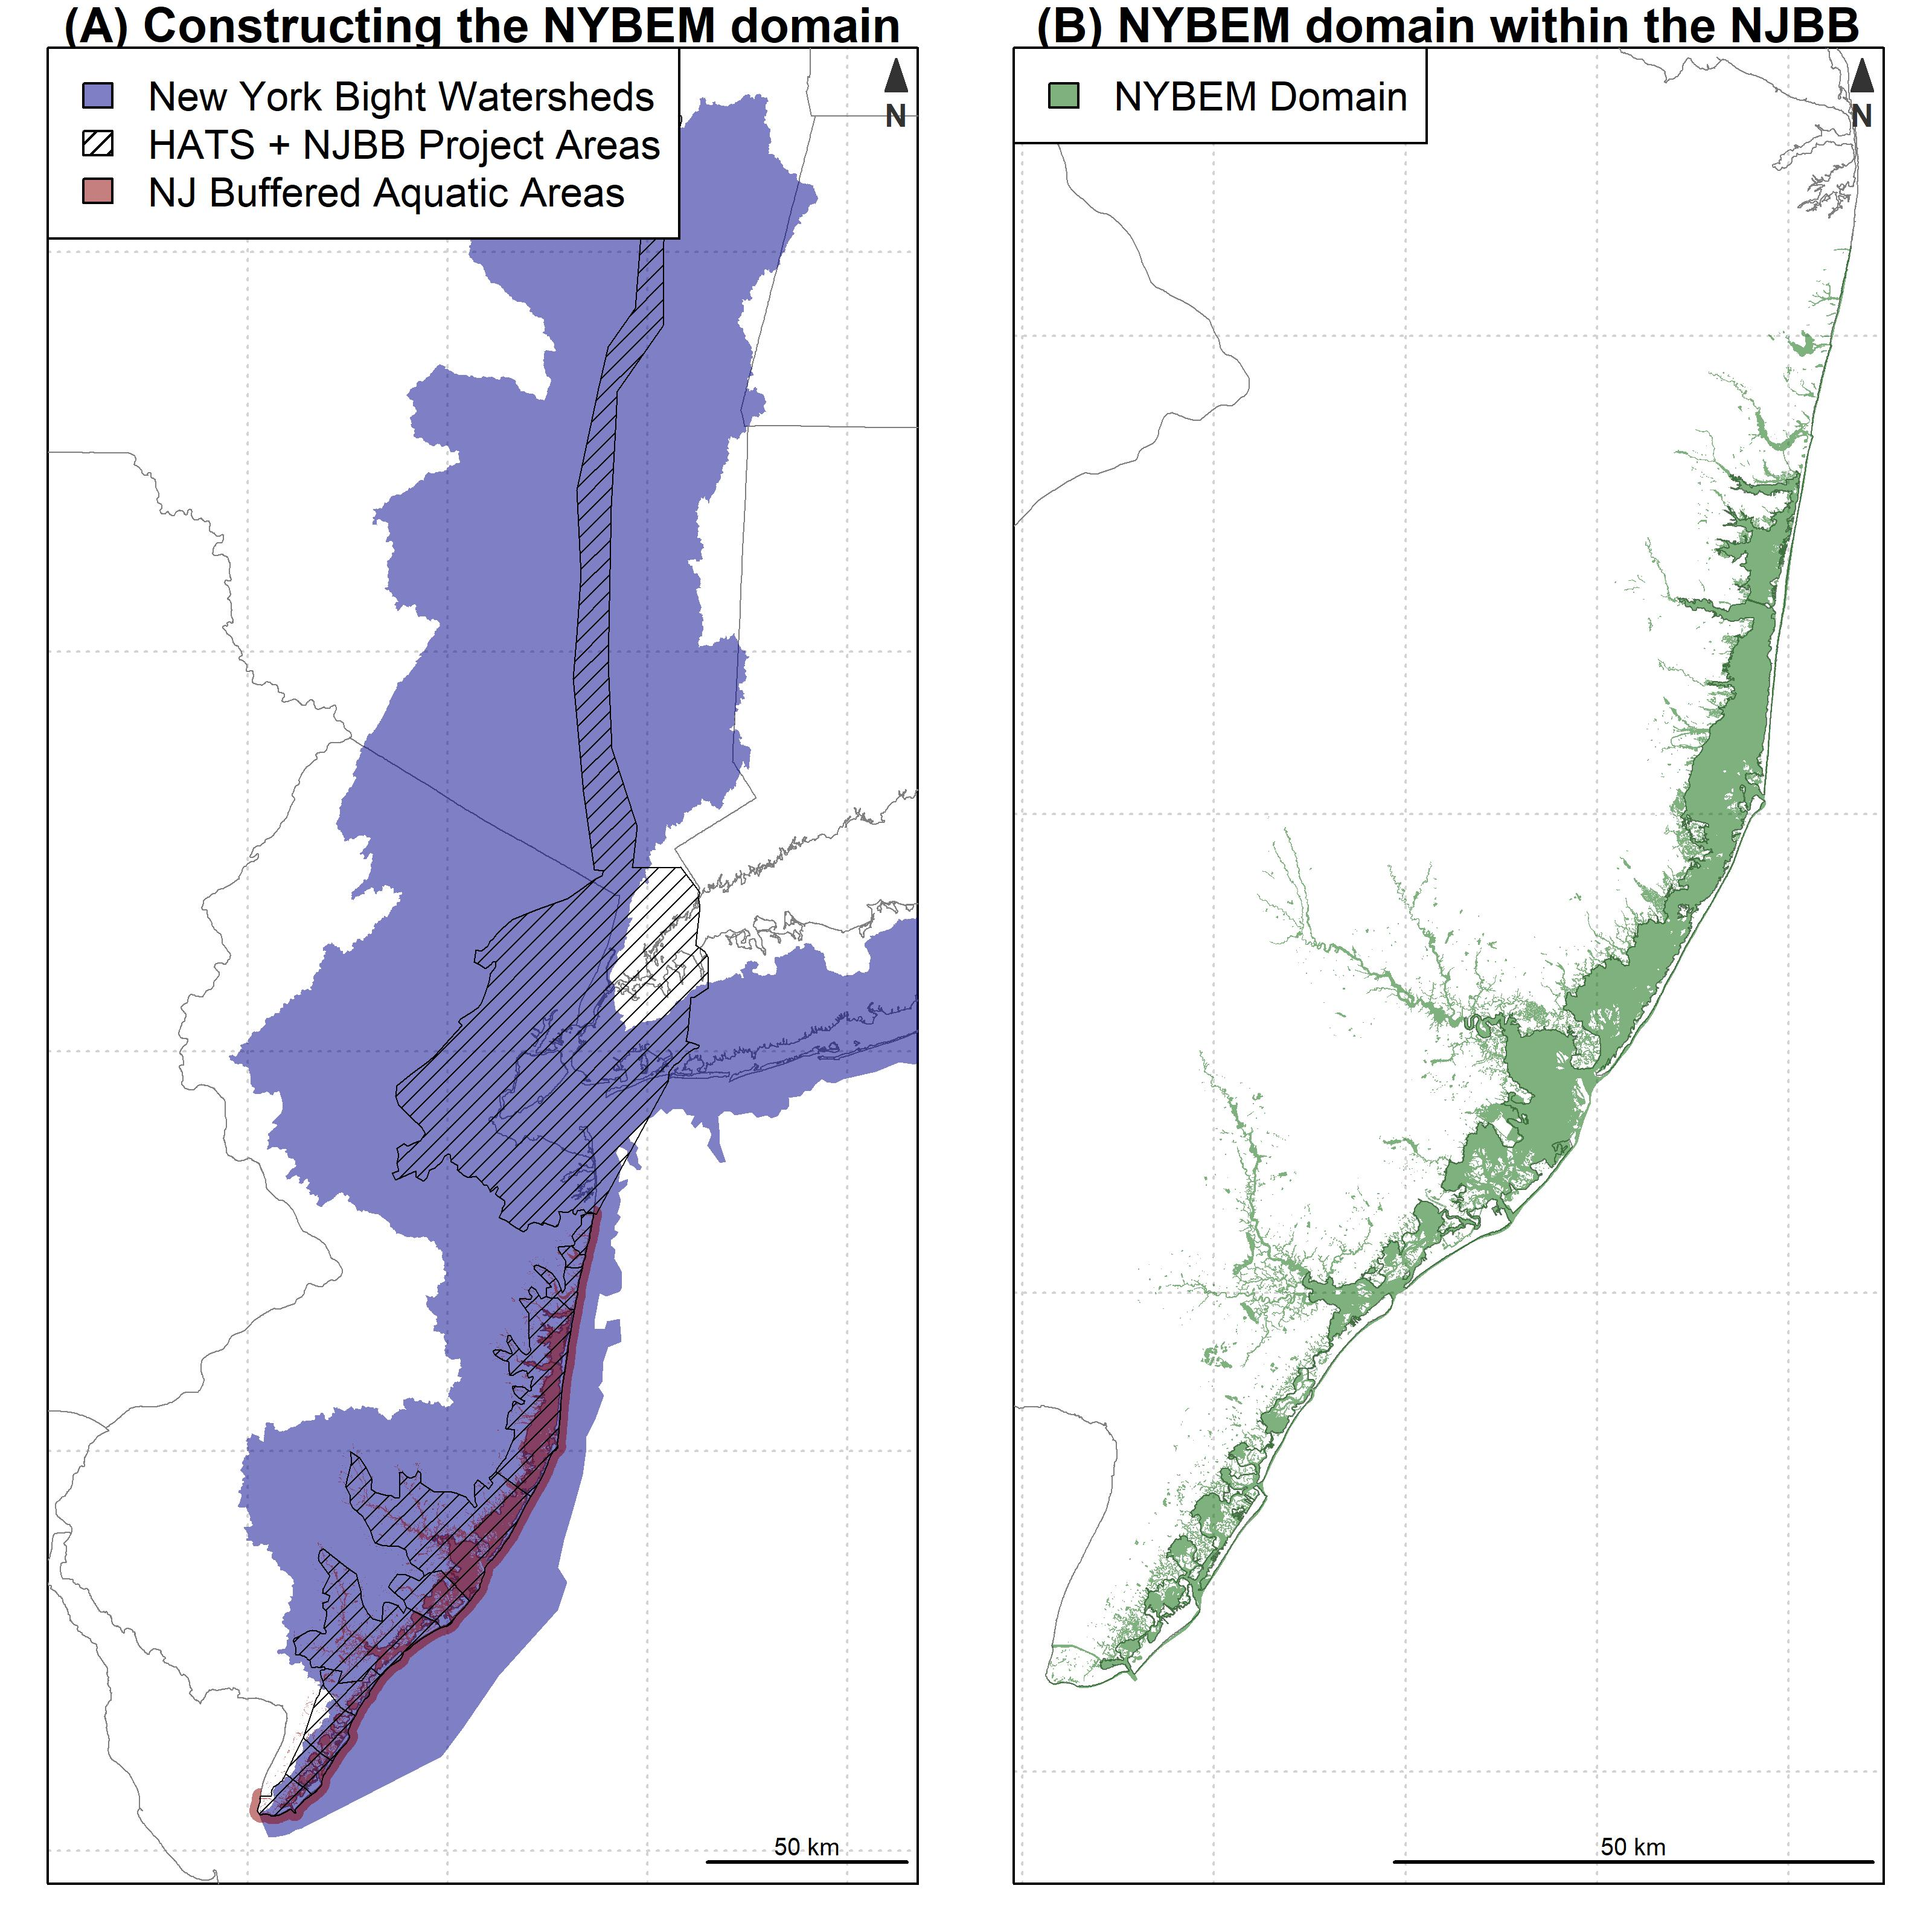
\includegraphics{ZZ_Fig02_NYBEM.Extent.jpeg}
\caption{\emph{Figure 2. NYBEM model domain: (left) Components of model domain, (right) NYBEM domain.}}
\end{figure}

\hypertarget{phased-approach}{%
\section{Phased Approach}\label{phased-approach}}

USACE planning studies sequentially make decisions about potential actions and buy-down risk and uncertainty to inform the next level of decision and narrow in on a recommended alternative. Furthermore, the USACE studies have proposed a ``tiered'' NEPA assessment, which is designed to gather more data and refine outcomes as a project proceeds. The NYBEM toolkit must be capable of responding to evolving project planning needs and data availability as these studies develop. As such, model development is explicitly being conducted in ``phases,'' and NYBEM tools and methods will evolve alongside project planning. In each phase, development will proceed iteratively through the cycle described above of conceptualization, quantification, evaluation, application, and communication. Table 1 presents key aspects of this phased approach to development.

Importantly, a phased development approach applies the best available information at the moment of application. However, this inherently leads to ``interim'' or ``draft'' models that are sequentially applied, reviewed, and improved. In this report, Phase 1 of model development is documented, while presenting the planned path forward for future phases. Development plans are subject to change.

\begin{table}

\caption{\label{tab:unnamed-chunk-3}Table 1. Phased approach to development of the NYBEM.}
\centering
\begin{tabular}[t]{c|c|c|c}
\hline
District Planning Milestone & Interim Report & Draft Feasibility Report & Final Feasibility Report\\
\hline
Type of Decision & Preliminary Screening & Alternatives Analysis & Design and Operation of Recommended Alternative\\
\hline
Scope of Environmental Effects & Direct & Direct + Indirect & Direct + Indirect + Cumulative\\
\hline
Spatial Extent of Environmental Effects & Project footprint & Maximum extent of impacts & Mitigation requirements\\
\hline
Anticipated Outputs & Project footprint & Habitat Quantity (by type) & Habitat Quantity, Quality, and Connectivity (by type)\\
\hline
Analytical Effort & Rapid Screening & Moderate & Detailed\\
\hline
Hydraulic Forcing & Existing Condition & One year of tidal forcing + Multiple sea levels & Multiple years of tidal forcing + Multiple sea levels\\
\hline
Model Inputs & Footprint & Footprint + Tidal Range + Salinity & Footprint + Tidal Range + Salinity + Hydrodynamics + Sediment + Temperature + Waves + Water Quality + Other\\
\hline
\end{tabular}
\end{table}

\hypertarget{mediated-modeling}{%
\section{Mediated Modeling}\label{mediated-modeling}}

The NYBEM intends to assess ecological consequences of alternative infrastructure options in a large, diverse ecosystem. There are many types of stakeholder-based model development processes that overlap in approach and emphasize collaboration: Model Prototyping, Participatory Modeling, Group Model Building, Companion Modeling and Mediated Model Development \citetext{\citealp[See reviews by][]{voinov_modelling_2010}; \citealp{gray_environmental_2017}; \citealp[and][]{hall_mediated_2019}}. These processes are generally well-suited to environmental management problems that are politically and publicly-sensitive, complex, and engage diverse audiences \citep{van_den_belt_mediated_2006}. ``Mediated modeling'' is used here to describe the family of techniques for building consensus among multiple partners and producing credible and defensible ecological models in a transparent way \citep{van_den_belt_mediated_2006}.
For NYBEM, a suite of workshop-based model development methods are adapted from \citet{herman_unpacking_2019}. These workshops utilize a lecture-exercise format, where participants are led through the theory of a particular aspect of modeling (e.g., conceptual modeling) and then apply said theory to a focal ecosystem (i.e., the New York Bight). A series of workshops and reviews are structuring the iterative development of NYBEM with subsequent research and synthesis between meetings (See McKay et al.~2021 for additional detail). Appendix B summarizes workshop logistics and focal topics. Key milestones in model development are briefly described below, but the overarching strategy is to engage larger audiences and more formal forms of model evaluation as the toolkit develops.

\begin{itemize}
\item
  \emph{Preliminary workshop with Philadelphia District} (January 2019): A preliminary conceptual model was developed with USACE Philadelphia District team members, which focused generally on issues potentially relevant for environment compliance at the broadest level.
\item
  \emph{USACE workshop with Philadelphia and New York Districts} (March 2019): A joint team from multiple USACE Districts was convened, and a strategy was proposed to develop NYBEM around key ecosystem types to reduce the dimensionality and complexity of the modeling problem and structure the path forward for model development.
\item
  \emph{Interagency conceptual modeling workshop} (June 2019): Fifty scientists and environmental managers (from federal, state, and local government as well as select non-profit organizations and academic units) were brought together to focus on the development of conceptual models supporting the NYBEM. This workshop utilized a series of ``posters'' for attendees to provide input on relevant variables and processes for each ecosystem type.
\item
  \emph{Interagency numerical modeling workshop} (November 2019): A subset of attendees (20+) from the June 2019 workshop reconvened to discuss findings from the prior workshops. Prior to this meeting, the ``posters'' from June were formalized and synthesized with available scientific literature. At this meeting, attendees were able to review and revise preliminary versions of the model structure.
\item
  \emph{Phase-1 model documentation} (March 2022; this report): This report provides model development status as of the NJBB Draft Feasibility Report and Environmental Impact Statement.
\item
  \emph{Phase-2 development and application} (Summer 2022): Habitat quality and system connectivity tools will be further developed following the release of the Draft NJBB Feasibility Report. USACE requires assessment and external evaluation of ecological models used in Feasibility-level planning decisions (i.e., model certification), and this report will be modified as models are further developed and applied.
\end{itemize}

Rapid timelines and iterative development encourage a transparent approach for model documentation. We adopt a growing family of methods for ``\href{https://ropensci.github.io/reproducibility-guide/sections/introduction/}{reproducible research},'' which embrace code and data sharing, enable review processes, and facilitate use of methods and results. Specifically, \href{https://rmarkdown.rstudio.com/}{R Markdown} is applied to development and document models, which are coded in the \href{https://cran.r-project.org/}{R Statistical Software}. These tools minimize data transfer errors and facilitate internal inspect of code as it is developed.

\hypertarget{conceptualization}{%
\chapter{Conceptualization}\label{conceptualization}}

The foundation of ecological modeling is a clear conceptualization of the ecosystem and an approach for translating the conceptual model into a numerical representation. This chapter describes an overarching conceptual model for the ecosystems of the New York Bight. A strategy is then presented for assessing these ecosystems relative to a habitat-style modeling approach, where the quantity and quality of each ecosystem type are computed separately and combined into an index of ecosystem integrity (i.e., a ``habitat unit'').

\hypertarget{conceptual-model}{%
\section{Conceptual Model}\label{conceptual-model}}

Conceptual ecological models are required for all USACE ecosystem restoration projects due to their utility to increase understanding, identify potential alternatives, and facilitate team dialog \citep{fischenich_application_2008, us_army_corps_of_engineers_assuring_2011}. These same benefits apply for assessing environmental effects of proposed coastal storm risk management actions. Additionally, conceptual models also inform and structure the development of quantitative ecological models \citep{grant_ecological_2008, swannack_ecological_2012} such as the NYBEM. Conceptual models of the New York Bight were iteratively developed through the mediated workshops described in Section 2.3. Workshop ideas and content were synthesized with available literature, conceptual models of similar ecosystems (e.g., wetland function in Coastal Louisiana; \citet{twilley_formulation_nodate}), and existing regional conceptual models \citep[e.g.,][]{montagna_conceptual_2013}. A seven step conceptual model development process was iteratively applied as workshops proceeded {[}\citet{fischenich_application_2008}; Table 3.1{]}.

\begin{table}

\caption{\label{tab:unnamed-chunk-4}Stepwise development of the overarching NYBEM conceptual model (following steps in Fischenich 2008).}
\centering
\begin{tabu} to \linewidth {>{\raggedright}X>{\raggedright}X}
\hline
Step & NYBEM Application\\
\hline
1. State the model objectives. & Our numerical modeling objective is to articulate the mechanisms and magnitude of environmental effects of proposed coastal storm risk management actions in the New York Bight Ecosystem. This conceptual model is intended to communicate the overarching scope of model development to a broad audience.\\
\hline
2. Bound the system of interest. & NYBEM is limited to the New York Bight Watershed with a seaward limit of a 20m depth contour. The models are further limited to aquatic ecosystems within the NJBB and HATS project areas. The NYBEM focuses only on effects to regional ecosystem, and other forms of environmental impacts (e.g., air quality, historic preservation) are addressed elsewhere in NEPA documentation.\\
\hline
3. Identify critical model components within the system. & This overarching conceptual model focuses on key ecosystem types and system-wide connectivity. Patch-scale models are defined from a combined classification based on Cowardin et al. (1979), USFWS (1997), and Montagna et al. (2013). A series of workshops and literature search were then used to identify ecosystem-specific model components associated with habitat quality (Chapter 4).\\
\hline
4. Articulate relationships among model components. & Only ecosystem types are presented, given the communication-driven purpose of this overarching model. More mechanistic conceptual models are presented for each ecosystem type ub Chapter 4, which show connections between drivers and stressors, ecosystem states, and ecological outcomes.\\
\hline
5. Represent the conceptual model. & A simple graphic representation of the conceptual model (Figure 3.1) was developed to facilitate communication between project team members, sponsors, partner agencies, and other interested parties.\\
\hline
6. Describe the expected pattern of behavior. & The team qualitatively assessed the model along with potential gaps in ecosystem types and environmental impacts.\\
\hline
7. Test, review, and revise. & This overarching conceptual model was developed, presented, and refined based on a series of modeling workshops over a three year timeframe.\\
\hline
\end{tabu}
\end{table}

Ultimately, multiple conceptual models were developed of the New York Bight with different purposes. We first developed an overarching conceptual model communicating how a mosaic of regional ecosystems function together at a system-scale, which is intended for broad use including both technical and non-technical audiences (Figure 3.1). Three overarching systems were identified to frame model development: (1) nearshore / marine ecosystems, (2) estuarine ecosystems, and (3) system connectivity between multiple ecosystem types. These systems were distinguished based on differences in ecosystem processes such as wave energy and salinity dynamics, likely effects of proposed management alternatives, and potential differences in modeling philosophy (e.g., habitat models for nearshore and estuarine systems and a network approach to connectivity). Cumulatively, these three categories provide a means of assessing nearshore and estuarine ecosystems at a patch-scale as well as a means of assessing system-scale outcomes associated with connectivity. The ecosystem types were adopted from a combination of two existing classifications \citep{cowardin_classification_1979, us_fish_and_wildlife_service_usfws_significant_1997}. In addition to this overarching model, mechanistic conceptual models were developed for each ecosystem type to guide quantitative model development (see Chapter 4), which are intended for technical audiences focused on the scientific details of ecological assessments.

\begin{figure}
\centering
\includegraphics{ZZ_Fig03_NYBEM.ConModel.jpg}
\caption{\emph{Overarching conceptual model for the New York Bight.}}
\end{figure}

\hypertarget{major-ecosystem-types}{%
\section{Major Ecosystem Types}\label{major-ecosystem-types}}

Patch-scale assessments were developed for both the marine and estuarine ecosystems. Models were developed for each of six major ecosystem types (Table 3.2). These ecosystems are defined from a combined classification based on \citet{cowardin_classification_1979} and \citet{us_fish_and_wildlife_service_usfws_significant_1997}. Salinity and tidal range differentiate these ecosystems, both of which can change under futures with and without agency projects. Other analyses have developed ecosystem-scale assessments and models based on similar or more refined divisions in physical properties (e.g., \citet{clough_modeling_2016}, \citet{fischbach_building_2018}), and the current criteria represent a compromise between the need for detailed assessment of the type and location of infrastructure impacts and the need for a readily implementable rule set applicable at the broad spatial scale of the NYBEM.

\begin{table}

\caption{\label{tab:unnamed-chunk-5}Definition of NYBEM ecosystem types.}
\centering
\begin{tabu} to \linewidth {>{\raggedright}X>{\raggedright}X>{\raggedright}X>{\raggedright}X}
\hline
Tidal Limits & Marine (Salinity >= 30ppt) & Estuarine (Salinity = 0.5 to 30ppt) & Freshwater (Salinity <= 0.5ppt)\\
\hline
Deepwater (-2m to -20m) & Marine, Deep & Estuarine, Subtidal & Freshwater\\
\hline
Subtidal (MLLW to -2m) & Marine, Subtitdal & Estuarine, Subtidal & Freshwater\\
\hline
Intertidal (MHHW to MLLW) & Marine, Intertidal & Estuarine, Intertidal & Freshwater\\
\hline
\end{tabu}
\end{table}

\hypertarget{habitat-style-modeling-philosophy}{%
\section{Habitat-Style Modeling Philosophy}\label{habitat-style-modeling-philosophy}}

Dozens of ecological modeling tools focus on coastal ecosystems. These models vary based on factors such as the disciplinary perspective (e.g., hydrologic, geomorphic, ecological), the level of ecological hierarchy addressed (e.g., individuals, populations, communities, ecosystems), the basic approach to modeling (e.g., statistical, theoretical), input requirements (e.g., few parameters vs.~extensive geospatial layers), the treatment of time and space (e.g., lumped vs.~distributed), and the degree of development (e.g., long history vs.~ad hoc). However, multiple gaps in these these tools are the driving motivation for developing the New York Bight Ecological Model (NYBEM).

\begin{itemize}
\tightlist
\item
  \emph{Comprehensive view of regional ecosystems}: Many existing ecological models focus on a subset of regional ecosystems (e.g., estuarine subtidal, but not marine subtidal) or focal taxa (e.g., fish, but not seagrass). The large spatial scope of the USACE studies requires seamless landscape coverage of the study areas as well as a consistent approach for assessing multiple ecosystem types simultaneously.\\
\item
  \emph{Connection to USACE management actions}: Existing tools often emphasize important physical forcings on ecosystems without a direct connection to USACE's proposed project action. For instance, a model may include marsh response to sea level rise, but be unable to incorporate marsh response to sea level rise in the presence of a storm surge barrier.\\
\item
  \emph{Indirect effects}: Models often emphasize direct changes at a site-scale rather than indirect effects of off-site change. For instance, a model may assess habitat quality associated with substrate, but be unable to link to changes in substrate as a result of distant infrastructure (e.g., a storm surge barrier).\\
\item
  \emph{System-wide data}: Many valuable ecological tools have been developed at small spatial scales based on detailed site data (e.g., vegetation surveys or field assessment procedures). However, the extremely large scale of these projects precludes field data collection, and NYBEM inputs must be available for the entire model extent.\\
\item
  \emph{Rapid and phased application}: The USACE studies are assessing project outcomes within limited timeframes, and some tools that might be applicable on longer time horizons are not feasible in these short periods. Additionally, the projects require an evolving set of tools that mirror the needs of a tiered NEPA assessment.
\end{itemize}

Given these challenges, the NYBEM seeks to build from the wide breadth of existing knowledge and models to develop a comprehensive set of tools directly applicable to the unique needs of planning USACE coastal storm risk management projects. The NYBEM draws from two distinct modeling approaches applicable at different scales. First, six patch-scale models were developed, which use an index-based modeling philosophy assessing the quantity and quality of a given ecosystem type. Second, system-scale models will be developed in the future, which apply network-analytic methods to assess organismal connectivity. This report documents only the patch-scale models applicable in the six ecosystems shown in Table 3.2.

The NYBEM takes a common approach to ecological modeling based on quantity and quality of habitat. ``Index'' models \citep{swannack_ecological_2012} were originally developed for species-specific habitat applications (e.g., slider turtles), but the general approach has also been adapted to guilds (e.g., salmonids), communities (e.g., floodplain vegetation), and ecosystem processes (e.g., the Hydrogeomorphic Method). An index-based modeling approach is used for multiple reasons. First, index models directly respond to changes in physical properties and provide a clear link to changes in ecosystem quantity and quality resulting from future conditions with and without proposed actions. Second, index-based models align well with a phased model development approach. For instance, an initial model could use three critical variables influencing habitat quality, and future model versions could include more variables as data becomes available. Third, index-based models are familiar to USACE decision-makers from diverse applications in other regions such as Louisiana coastal restoration (i.e., the Wetland Value Assessment), California bay restoration (i.e., East San Pedro Bay), and Gulf Coast harbor expansion (i.e., Mobile Bay). Notably, these examples each assess multiple habitat types (e.g., oyster, seagrass) and aggregate outcomes into an overall metric of ecological impacts or benefits.

In NYBEM, the quantity and quality of each ecosystem type are assessed separately. For instance, ecosystem extent and habitat quantity is rapidly delineated from modeled hydrodynamic conditions. Ecosystem quality is then assessed based on patch-specific data and known thresholds in ecological response (e.g., on a normalized 0 to 1 scale indicating ecological quality or function). The product of habitat quality and quantity provides a consistent metric across ecosystem types (i.e., ``habitat units''). Here, the terms ``habitat'' and ``ecosystem'' are used synonymously to indicate a given patch.

\hypertarget{quantification}{%
\chapter{Quantification}\label{quantification}}

The quantification phase of ecological model development formalizes a conceptual model in terms of mathematical relationships, model parameters, and a numerical algorithm (Grant and Swannack 2008). This chapter describes the NYBEM relative to model structure, associated numerical tools, and the theoretical underpinnings of the sub-models. In general, the overarching quantitative architecture of the NYBEM can be summarized in three major elements (Figure 4.1). First, model inputs are assembled in a geospatial database. Second, the model code is prepared as a ``package'' in the \href{https://cran.r-project.org/}{R Statistical Software}. Finally, the model outputs habitat quantity and quality as well as habitat units for each patch in the model domain.

\begin{figure}
\centering
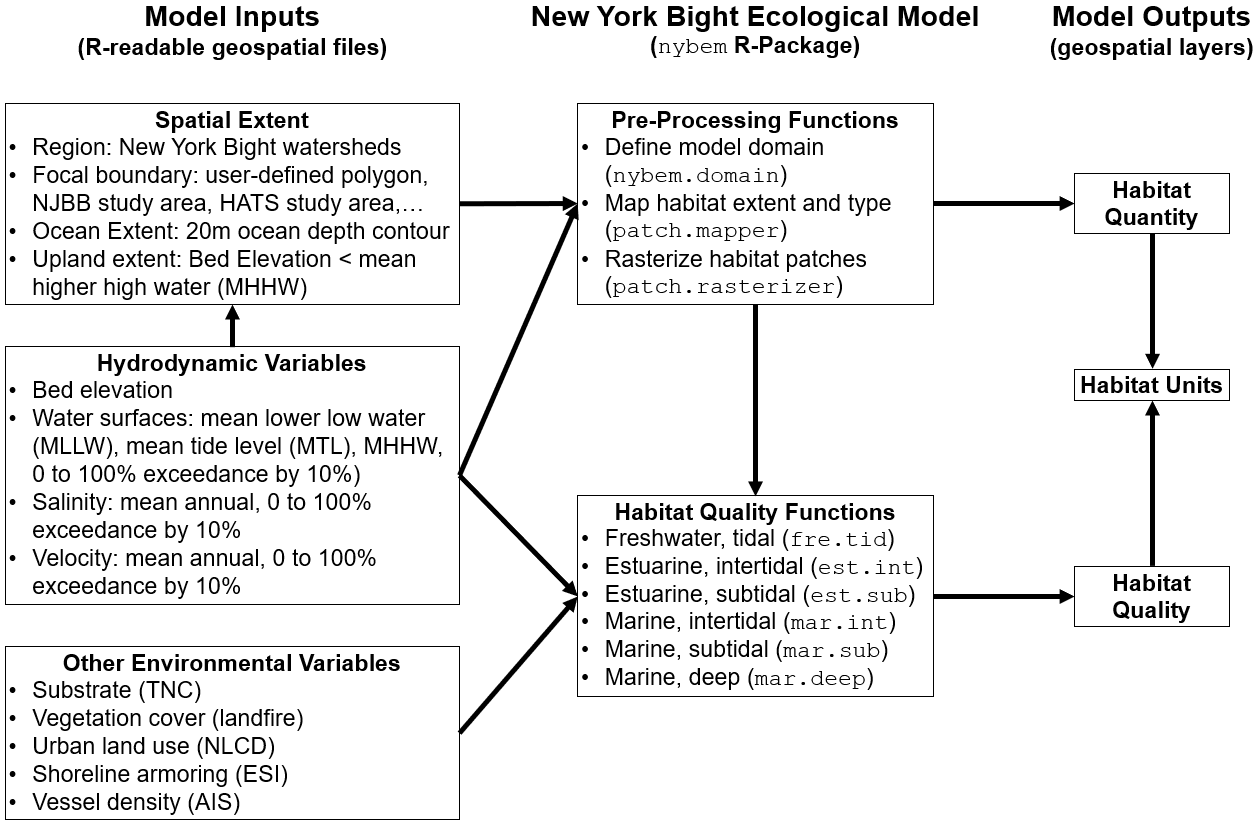
\includegraphics{ZZ_Fig04_NYBEM.Architecture.png}
\caption{\emph{Quantitative architecture of the NYBEM.}}
\end{figure}

Input variables to NYBEM consist of three major groups of data layers. First, the spatial extent of a given model run must be defined. The NYBEM is constrained to applications within the region of the New York Bight watersheds (Section 2.1). Within that region, a focal area for the simulation must be specified, which can consist of a particular project boundary (e.g., NJBB or HATS) or a user-specified domain (e.g., a particular back bay). Within that focal area, the downstream and upstream extents of the model are specified based on the 20m ocean depth contour and Mean Higher High Water (MHHW), respectively. The second major group of variables consists of hydrodynamic inputs. These inputs may be computed for varying temporal windows (e.g., a month, a year, or a decade) depending on the project focus, and the inputs could be provided by a variety of hydrodynamic models or empirical data sources. Hydrodynamic variables characterize the bed elevation, water surface, salinity, and velocity distributed throughout the project area. Third, a variety of other environmental variables are compiled from national and regional data sets to inform habitat quality calculations.

All model code for the NYBEM is contained within an R-package (\texttt{nybem}, \href{https://github.com/MVR-GIS}{available via github}). Generally speaking, a package can be thought of as a fundamental unit of code that can include functions, data, documentation, and tests (\href{https://r-pkgs.org/}{Wickham and Bryan 2019}). Packages then provide a transportable and reproducible mechanism for code sharing and publication. The \texttt{nybem} package contains nine functions and associated testing trials. This chapter describes each function in detail, but they can be summarized briefly as:

\begin{itemize}
\tightlist
\item
  \texttt{nybem.domain}: This function defines the model domain based on regional extent of the New York Bight watersheds, a user-specified focal area, a downstream extent of a 20m ocean depth contour, and an upstream extent based on bed elevations less than MHHW.\\
\item
  \texttt{patch.mapper}: This function maps the extent of NYBEM's six major ecosystem types (Table 3.2) based on user-specified data layers for bed elevation, MLLW, MTL, MHHW, and salinity.\\
\item
  \texttt{patch.rasterizer}: This function rasterizes the output of \texttt{patch.mapper} based on a specified grid resolution and aligns that layer with a specified spatial coordinate system.\\
\item
  \texttt{fre.tid}: This function computes habitat quality for any freshwater, tidal patches.\\
\item
  \texttt{est.int}: This function computes habitat quality for any estuarine, intertidal patches.\\
\item
  \texttt{est.sub}: This function computes habitat quality for any estuarine, subtidal patches.\\
\item
  \texttt{mar.int}: This function computes habitat quality for any marine, intertidal patches.\\
\item
  \texttt{mar.sub}: This function computes habitat quality for any marine, subtidal patches.\\
\item
  \texttt{mar.deep}: This function computes habitat quality for any marine, deepwater patches.
\end{itemize}

The first three functions can largely be thought of as pre-processing fundamental input data and mapping the extent of the six ecosystem types. For purposes of model development, these are relatively straight-forward and will be documented collectively. The latter six functions each compute a 0 to 1 metric of ecosystem condition (i.e., habitat quality) based on a unique set of input variables, equations, and parameters. Each of these habitat quality sub-models followed a consistent set of development steps, which are documented throughout this chapter and briefly describe here. Preliminary variables were identified at a series of interagency workshops through a series of conceptual modeling exercises (Appendix A). Additional variables were added based on taxa-specific habitat suitability models (i.e., USFWS ``blue books''), relevant tools (e.g., New England Marsh Model), and literature search. A conceptual model was then developed for each ecosystem type to better understand how key variables related an influenced each other. An overarching list of regional and national data sets were also compiled to assure that model variables could be assessed throughout the broad spatial extent of the New York Bight. Potential model variables were compiled along with the rationale for inclusion or exclusion. Finally, a numerical ``suitability index'' was developed for each variable remaining in the sub-model based on existing suitability indices, published thresholds / responses, and professional judgment.

Ultimately, the \texttt{nybem} allows users to assess the extent and integrity of the six major ecosystem types represented in the NYBEM. The size and quality of a given habitat patch can provide useful metrics in their own right, or they may be summarized as an overarching ``habitat unit'' (i.e., the quantity of habitat in acres * patch quality assessed on a 0 to 1 scale).

\hypertarget{pre-processing-functions-i}{%
\section{Pre-Processing Functions (I)}\label{pre-processing-functions-i}}

{Need Dougherty's help on this one.}

Insert pre-amble text. This chapter describes each function in detail, but they can be summarized briefly as:

\hypertarget{define-model-domain}{%
\subsection{Define Model Domain}\label{define-model-domain}}

\texttt{nybem.domain}: This function defines the model domain based on regional extent of the New York Bight watersheds, a user-specified focal area, a downstream extent of a 20m ocean depth contour, and an upstream extent based on bed elevations less than MHHW.

\begin{Shaded}
\begin{Highlighting}[]
\CommentTok{\#Functions for rasterizing habitat types}
\NormalTok{nybem.domain }\OtherTok{\textless{}{-}} \ControlFlowTok{function}\NormalTok{(NYBightWatersheds, Ocean20mDepth, bedelev, MHHW)\{}
  \CommentTok{\#Insert code}
\NormalTok{\}}
\end{Highlighting}
\end{Shaded}

\hypertarget{map-habitat-extent-and-type}{%
\subsection{Map Habitat Extent and Type}\label{map-habitat-extent-and-type}}

\texttt{patch.mapper}: This function maps the extent of NYBEM's six major ecosystem types (Table 3.2) based on user-specified data layers for bed elevation, MLLW, MTL, MHHW, and salinity.

In NYBEM, the quantity and quality of each ecosystem type may be assessed separately. For instance, ecosystems could be rapidly delineated from empirical data for the existing condition (e.g., field or tide gauge) or modeled hydrodynamic data for future conditions or proposed management actions. These delineated ecosystems can be summarized as an overarching habitat quantity in acres. Ecosystem quality may then be assessed based on patch-specific data and known thresholds in ecological response (e.g., on a normalized 0 to 1 scale indicating ecological quality or function). The product of habitat quality and quantity provides a consistent metric across ecosystem types (i.e., ``habitat units''). Here, the terms ``habitat'' and ``ecosystem'' are used synonymously to indicate a given patch.

The criteria for delineating ecosystems (Table 3) were subsequently programmed as a suite of logic statements for identifying the salinity zone, tidal zone, or ecosystem / habitat type for any given patch. The following functions input salinity, bed elevation, mean lower low water (MLLW), and mean higher high water (MHHW) and output a numerical code indicating salinity, tidal, and habitat zone as follows.

\begin{itemize}
\tightlist
\item
  \emph{Tidal Zone}: 1 = deep, 2 = subtidal, 3 = intertidal, and 4 = upland
\item
  \emph{Salinity Zone}: 1 = marine, 2 = estuarine, or 3 = freshwater\\
\item
  \emph{Habitat Zone / Ecosystem Type}: 1 = upland, 2 = marine, deepwater, 3 = marine, subtidal, 4 = marine, intertidal, 5 = estuarine subtidal, 6 = estuarine intertidal, or 7 = freshwater
\end{itemize}

\begin{Shaded}
\begin{Highlighting}[]
\CommentTok{\#Functions for isolating habitat types}

\DocumentationTok{\#\#\#\#\#\#\#\#\#\#}
\CommentTok{\#Labels for tidal zones}
\NormalTok{ZoneTidal }\OtherTok{\textless{}{-}} \FunctionTok{c}\NormalTok{(}\StringTok{"Deep"}\NormalTok{, }\StringTok{"Subtidal"}\NormalTok{, }\StringTok{"Intertidal"}\NormalTok{, }\StringTok{"Upland"}\NormalTok{)}

\CommentTok{\#Create function for isolating tidal zones}
\NormalTok{set.tidal.zone }\OtherTok{\textless{}{-}} \ControlFlowTok{function}\NormalTok{(bedelev, MLLW, MHHW)\{}
  \CommentTok{\#Assign zone}
\NormalTok{  tidalzone }\OtherTok{\textless{}{-}} \FunctionTok{ifelse}\NormalTok{(bedelev }\SpecialCharTok{\textless{}=} \SpecialCharTok{{-}}\DecValTok{2}\NormalTok{, }\DecValTok{1}\NormalTok{,}
          \FunctionTok{ifelse}\NormalTok{(bedelev }\SpecialCharTok{\textless{}=}\NormalTok{ MLLW, }\DecValTok{2}\NormalTok{,}
          \FunctionTok{ifelse}\NormalTok{(bedelev }\SpecialCharTok{\textless{}=}\NormalTok{ MHHW, }\DecValTok{3}\NormalTok{, }
          \FunctionTok{ifelse}\NormalTok{(bedelev }\SpecialCharTok{\textgreater{}}\NormalTok{ MHHW, }\DecValTok{4}\NormalTok{, }\ConstantTok{NA}\NormalTok{))))}
  \CommentTok{\#Send output}
\NormalTok{  tidalzone}
\NormalTok{\}}

\DocumentationTok{\#\#\#\#\#\#\#\#\#\#}
\CommentTok{\#Labels for salinity zones}
\NormalTok{ZoneSalinity }\OtherTok{\textless{}{-}} \FunctionTok{c}\NormalTok{(}\StringTok{"Marine"}\NormalTok{, }\StringTok{"Estuarine"}\NormalTok{, }\StringTok{"Fresh"}\NormalTok{)}

\CommentTok{\#Create function for isolating salinity zones}
\NormalTok{set.salinity.zone }\OtherTok{\textless{}{-}} \ControlFlowTok{function}\NormalTok{(salinity)\{}
  \CommentTok{\#Assign zone}
\NormalTok{  salinityzone }\OtherTok{\textless{}{-}} \FunctionTok{ifelse}\NormalTok{(salinity }\SpecialCharTok{\textgreater{}=}\DecValTok{30}\NormalTok{, }\DecValTok{1}\NormalTok{, }
                  \FunctionTok{ifelse}\NormalTok{(salinity }\SpecialCharTok{\textless{}} \DecValTok{30} \SpecialCharTok{\&}\NormalTok{ salinity }\SpecialCharTok{\textgreater{}=} \FloatTok{0.5}\NormalTok{, }\DecValTok{2}\NormalTok{, }
                  \FunctionTok{ifelse}\NormalTok{(salinity }\SpecialCharTok{\textless{}} \FloatTok{0.5} \SpecialCharTok{\&}\NormalTok{ salinity }\SpecialCharTok{\textgreater{}=} \DecValTok{0}\NormalTok{, }\DecValTok{3}\NormalTok{, }\ConstantTok{NA}\NormalTok{)))}
  \CommentTok{\#Send output}
\NormalTok{  salinityzone}
\NormalTok{\}}

\DocumentationTok{\#\#\#\#\#\#\#\#\#\#}
\CommentTok{\#Labels for habitat zones}
\NormalTok{ZoneHabitat }\OtherTok{\textless{}{-}} \FunctionTok{c}\NormalTok{(}\StringTok{"Upland"}\NormalTok{, }\StringTok{"Marine.Deep"}\NormalTok{, }\StringTok{"Marine.Subtidal"}\NormalTok{, }\StringTok{"Marine.Intertidal"}\NormalTok{, }\StringTok{"Estuarine.Subtidal"}\NormalTok{, }\StringTok{"Estuarine.Intertidal"}\NormalTok{, }\StringTok{"Freshwater"}\NormalTok{)}

\CommentTok{\#Create function for isolating habitat zones}
\NormalTok{set.habitat.zone }\OtherTok{\textless{}{-}} \ControlFlowTok{function}\NormalTok{(tidalzone, salinityzone)\{}
  \CommentTok{\#Assign zone}
\NormalTok{  habitatzone }\OtherTok{\textless{}{-}} \FunctionTok{ifelse}\NormalTok{(tidalzone }\SpecialCharTok{==} \DecValTok{4}\NormalTok{, }\DecValTok{1}\NormalTok{,}
          \FunctionTok{ifelse}\NormalTok{(salinityzone }\SpecialCharTok{==} \DecValTok{1} \SpecialCharTok{\&}\NormalTok{ tidalzone }\SpecialCharTok{==} \DecValTok{1}\NormalTok{, }\DecValTok{2}\NormalTok{,}
          \FunctionTok{ifelse}\NormalTok{(salinityzone }\SpecialCharTok{==} \DecValTok{1} \SpecialCharTok{\&}\NormalTok{ tidalzone }\SpecialCharTok{==} \DecValTok{2}\NormalTok{, }\DecValTok{3}\NormalTok{,}
          \FunctionTok{ifelse}\NormalTok{(salinityzone }\SpecialCharTok{==} \DecValTok{1} \SpecialCharTok{\&}\NormalTok{ tidalzone }\SpecialCharTok{==} \DecValTok{3}\NormalTok{, }\DecValTok{4}\NormalTok{,}
          \FunctionTok{ifelse}\NormalTok{(salinityzone }\SpecialCharTok{==} \DecValTok{2} \SpecialCharTok{\&}\NormalTok{ tidalzone }\SpecialCharTok{==} \DecValTok{1} \SpecialCharTok{|}\NormalTok{ tidalzone }\SpecialCharTok{==} \DecValTok{2}\NormalTok{, }\DecValTok{5}\NormalTok{,}
          \FunctionTok{ifelse}\NormalTok{(salinityzone }\SpecialCharTok{==} \DecValTok{2} \SpecialCharTok{\&}\NormalTok{ tidalzone }\SpecialCharTok{==} \DecValTok{3}\NormalTok{, }\DecValTok{6}\NormalTok{,}
          \FunctionTok{ifelse}\NormalTok{(salinityzone }\SpecialCharTok{==} \DecValTok{3} \SpecialCharTok{\&}\NormalTok{ tidalzone }\SpecialCharTok{==} \DecValTok{1} \SpecialCharTok{|}\NormalTok{ tidalzone }\SpecialCharTok{==} \DecValTok{2} \SpecialCharTok{|}\NormalTok{ tidalzone }\SpecialCharTok{==} \DecValTok{3}\NormalTok{, }\DecValTok{7}\NormalTok{, }\ConstantTok{NA}\NormalTok{)))))))}
  \CommentTok{\#Send output}
\NormalTok{  habitatzone}
\NormalTok{\}}
\end{Highlighting}
\end{Shaded}

\hypertarget{rasterize-habitat-patches}{%
\subsection{Rasterize Habitat Patches}\label{rasterize-habitat-patches}}

\texttt{patch.rasterizer}: This function rasterizes the output of \texttt{patch.mapper} based on a specified grid resolution and aligns that layer with a specified spatial coordinate system.

\begin{Shaded}
\begin{Highlighting}[]
\CommentTok{\#Functions for rasterizing habitat types}
\NormalTok{patch.rasterizer }\OtherTok{\textless{}{-}} \ControlFlowTok{function}\NormalTok{(patch.mapper.output, grid.resolution, my.coordinate.system)\{}
  \CommentTok{\#Insert code}
\NormalTok{\}}
\end{Highlighting}
\end{Shaded}

\hypertarget{freshwater-tidal-submodel-fresh.tid-i}{%
\section{Freshwater, Tidal Submodel (fresh.tid) (I)}\label{freshwater-tidal-submodel-fresh.tid-i}}

{Mahan and McKay to edit text.}

1-2 paragraphs providing background on the ecosystem type. Physical properties. Typical ecological functions and ecosystem services.

Present and describe the conceptual model for this system.

\emph{START PARAGRAPH HERE}

\textbf{FIGURE}

Describe the main ideas being captured in the model. Summarize as table. Present suitability index curves, which are described in subsequent sections.

\textbf{TABLE}

\textbf{FIGURE WITH SUITABILITY CURVES}

Present the overarching habitat suitability index equation.

\textbf{EQUATION}

\hypertarget{variable-1}{%
\subsection{Variable-1}\label{variable-1}}

2-5 paragraphs presenting three main ideas.

Provide some general context for this variable's role in ecosystem function and condition.

Describe how this variable is assessed and quantified in NYBEM.

Present the equation for assessing the suitability index.

\textbf{EQUATION}

\hypertarget{variable-1-1}{%
\subsection{Variable-1}\label{variable-1-1}}

2-5 paragraphs presenting three main ideas.

Provide some general context for this variable's role in ecosystem function and condition.

Describe how this variable is assessed and quantified in NYBEM.

Present the equation for assessing the suitability index.

\textbf{EQUATION}

\hypertarget{fresh.int-code}{%
\subsection{fresh.int Code}\label{fresh.int-code}}

Numerical code for assessing habitat quality ({Dougherty and McKay to write.})

\begin{Shaded}
\begin{Highlighting}[]
\CommentTok{\#Function for assessing habitat quality}
\NormalTok{fresh.tid }\OtherTok{\textless{}{-}} \ControlFlowTok{function}\NormalTok{(x, y)\{}
\NormalTok{  fresh.tid.HSI }\OtherTok{\textless{}{-}}\NormalTok{ x }\SpecialCharTok{+}\NormalTok{ y}

  \CommentTok{\#Send output}
\NormalTok{  fresh.tid.HSI}
\NormalTok{\}}
\end{Highlighting}
\end{Shaded}

\hypertarget{estuarine-intertidal-submodel-est.int-i}{%
\section{Estuarine, Intertidal Submodel (est.int) (I)}\label{estuarine-intertidal-submodel-est.int-i}}

{Mahan and McKay to write.}

Estuarine environments include marine water that has been diluted by freshwater runoff from the land \citep{prosser_impacts_2018}. Due to tidal influence, intertidal ecosystems are found between high and low tide, experiencing varying land and sea influences, whereas subtidal ecosystems are constantly submerged. The estuarine intertidal ecosystem considers areas with salinity values greater than 0.5 ppt to 30 ppt and elevation from MHHW to MLLW. Plant, animal, and microorganism populations, as well as their nonliving surroundings, interact as a working unit in intertidal ecosystems, which are exposed at low tides (Citation). Within the estuarine intertidal ecosystem, ecological processes are linked to physical and chemical characteristics. These characteristics can experience change under anthropogenic and climatic pressures that deviate from the homeostasis, or baseline, habitat condition. This can result in reduced habitat suitability across the estuarine intertidal ecosystem.

Tidal marshes are vegetated intertidal ecosystems found at the land-sea interface that serve as crucial transition zones for marine, freshwater, and terrestrial processes \citep{colombano_climate_2021}. Tidal marshes originated in a range of coastal and estuarine environments, and their location exposes them to a number of environmental factors (e.g., ocean currents, watershed hydrology) and environmental gradients (e.g., salinity)(Lauchlan and Nagelkerken 2020). Broad-scale climatic changes are already affecting the timing, size, and duration of naturally varying environmental variables in estuarine, and freshwater settings. Understanding the changes in environmental stressors from climate change and sea level rise (SLR) on the tidal marsh ecosystem is critical to evaluate changes after the addition of storm surge barriers.

The following variables are accessible to the estuarine intertidal submodel portion of the NYBEM: salinity, episodic sediment deposition, edge erosion, vegetative cover, development of adjacent uplands, and the presence/absence of shoreline armoring.

Present and describe the conceptual model for this system.

\textbf{FIGURE}

Describe the main ideas being captured in the model. Summarize as table. Present suitability index curves, which are described in subsequent sections.

\textbf{TABLE}

\textbf{FIGURE WITH SUITABILITY CURVES}

Present the overarching habitat suitability index equation.

\textbf{EQUATION}

\hypertarget{salinity}{%
\subsection{Salinity}\label{salinity}}

Salinity affects physical and chemical processes such as flocculation and the amount of dissolved oxygen (DO) in the water column, as well as the types of organisms that may exist in an estuary (Citation). Estuarine organisms have evolved to cope with salinity fluctuations. Those that prefer fresher water at the upstream river end of the estuary to species that prefer saltier water at the downstream sea end usually form a gradient. Estuarine plants and animals suffer when extremely high salinities persist for lengthy periods of time. During instances of heavy freshwater inflows from rivers, harm might also occur. Extreme events are the issue in both scenarios.

Higher salinity, lower nutrient intake, and lower sediment inputs associated with extremely low river inflow can stress or kill plants and animals, limit productivity owing to nutritional deficiency, and destroy marshes due to low sediment input. Low estuary salinity kills marine creatures when river inflow is extremely high; excessive nutrient inputs contribute to algae blooms; and increased sediment input suffocates sea grasses and oysters \citep{hopkinson_lateral_2018}.

The NYBEM estuarine intertidal submodel relies on a percent in deviation of salinity regime to represent change in tidal inundation and freshwater flow input across the ecosystem. As the percentage of deviation from the baseline salinity regime increases, habitat suitability for taxa within the estuarine intertidal ecosystem will decrease.

Present the equation for assessing the suitability index.

\textbf{EQUATION}

\hypertarget{edge-erosion}{%
\subsection{Edge Erosion}\label{edge-erosion}}

Climate change, pollution, and other anthropogenic effects are putting more pressure on terrestrial and marine ecosystems. Coastal flooding and shoreline erosion will likely become more common as sea levels rise and storm surges shift as a result of climate change. There is fear that tidal wetlands will drown as sea levels rise and sediment supplies to the shore decline across the world. Marsh sediment budgets are a geographically integrated measure of opposing constructive and destructive forces: a surplus of sediment can lead to vertical growth and/or lateral expansion, while a shortfall can lead to drowning and/or lateral contraction \citep{ganju_spatially_2017}. Many estuarine marshes face sediment deficits along the shoreline as a result of increased edge erosion. Edge degradation causes morphological changes that make it easier for waves to propagate to the marsh borders and promote the resuspension and export of sediments from the estuary \citep{li_wave-driven_2019}.

The percent change in edge erosion throughout the estuarine intertidal ecosystem is used to represent habitat suitability. When the percentage of shear stress for erosion is 10\% or greater, erosion occurs, resulting in a reduction in total marsh area and an increase in open water area. At a rate of 30\% shear stress from erosion, the habitat will no longer be suitable (habitat suitability equals zero.

Present the equation for assessing the suitability index.

\textbf{EQUATION}

\hypertarget{vegetation-cover}{%
\subsection{Vegetation Cover}\label{vegetation-cover}}

Vegetation provides various ecological services within the estuarine intertidal ecosystem, including providing a fish nursery environment, feed for migratory birds, nutrient cycling, carbon storage, and sediment stability, therefore reductions of vegetative cover can have a significant impact on shallow marine ecosystems. Seagrass meadows are disappearing at an alarming rate in shallow coastal and estuary marine environments, with losses similar to tropical rainforests, mangroves, and coral reefs due to anthropogenic and climate stress \citep{walter_large-scale_2020}.

The loss of vegetative cover changes the dynamics near the seabed in locations where there was formerly vegetation, and transforms huge areas of the estuary from a deposition and accretion-friendly environment to one that favors suspension and erosion. For estuaries, such high amounts of suspended particles and sediment-associated nutrients create a variety of environmental management issues. These include alterations in invertebrate and macrophyte populations as well as a general deterioration of aquatic environments \citep{cotton_effects_2006}.

For the NYBEM, habitat suitability increases as the percentage of vegetative cover increases throughout the habitat. When vegetative cover is equal to 100 percent, the estuarine intertidal ecosystem will have a high suitability value (greater than 90\%).

Present the equation for assessing the suitability index.

\textbf{EQUATION}

\hypertarget{episodic-sediment-deposition}{%
\subsection{Episodic Sediment Deposition}\label{episodic-sediment-deposition}}

Estuaries are efficient sediment traps where near-bottom circulation causes sediment flow convergence during the transition from brackish to fresh water, resulting in local maxima in suspended sediment concentration (SSC) and deposition rates. Marine materials are deposited from the continental shelf into estuarine habitats. Due to disparities in tidal currents (ebb versus flood tide), sediments are carried to supply sediment on varying timeframes. In the estuarine intertidal ecosystem, sediment transport capacity is mostly determined by river discharge and by the timing of discharge events in relation to the spring--neap cycle and subtidal oscillations in sea level \citep{prosser_impacts_2018}.

Due to the retreat of the salinity intrusion and increasing bed pressures, sediment deposition episodes can induce considerable bed resuspension in the estuary. These periodic flood and storm events are major drivers in sediment dynamics and contribute disproportionately to the total sediment discharge \citep{ralston_sediment_2013}. The duration of high-discharge episodes in relation to the estuarine reaction time, a feature that fluctuates seasonally with discharge and estuarine length, also affects sediment transport capacity \citep{palinkas_sediment_2014}. These short-term events can cause changes in the local biological community and affect seabed stability and strength.

In coastal and estuary environments across the world, harmful algal blooms (HABs) have substantial economic, public health, and ecological consequences. The influx of additional nutrients following an episode of sediment deposition have been known to cause harmful algal blooms (HABs)\citep{ralston_temperature_2014}. Further, the frequent upturn of sediment can displace biological organisms. The most significant foreshore processes for the horseshoe crab are episodic storms, which impact erosion and accretion cycles, swash and wave processes, which affect sediment mixing and activation, and tides, which affect water infiltration and exfiltration through the sediment \citep{nancy_jackson_armoring_2010}. During storms, erosion of the shoreline can result in the removal of material from the upper foreshore and deposition on the lower foreshore, or the foreshore moving horizontally landward.

The NYBEM estuarine intertidal submodel utilizes a depth threshold that represents optimal episodic sediment deposit levels. Sediment supply is a key determinant of long-term marsh stability. The percent of time the estuarine depth is greater than MHHW is an indicator of habitat suitability.

Present the equation for assessing the suitability index.

\textbf{EQUATION}

\hypertarget{developement-of-adjacent-upland}{%
\subsection{Developement of Adjacent Upland}\label{developement-of-adjacent-upland}}

The development of uplands within a watershed can have a direct and indirect impact on a variety of essential aspects in estuarine intertidal ecosystems. The combination of coastal erosion and upland development causes a ``coastal squeeze,'' in which low-lying, intertidal regions that would usually recede inland in the face of sea-level rise are diminished because man-made structures (e.g.~shoreline armoring) prevent such retreat \citep{prosser_impacts_2018}. This means that tidal marshes will need to shift upslope onto nearby uplands to survive in a period of rapid sea-level rise. Further, the top boundary of this migratory zone's tidal inundation is very unpredictable over time and may be rising faster than mean sea level. Land management methods on the tidal marsh's upland border can help or hinder ecosystem migration in response to increasing sea levels \citep{anisfeld_upslope_2017}.

Both developed and undeveloped uplands can experience ecological stress as a result of climate change and land use changes (e.g.~addition of storm surge barriers, shoreline armoring). Climate change's effects on ocean and watershed systems are intertwined and set to interact. This is especially true in tidal marshes, which are biogenic environments that are sculpted by tidal and fluvial processes and are dynamic and architecturally complex \citep{colombano_climate_2021}. Multiple stressors can affect the development of adjacent uplands such as low-flows, flooding, and reduced stream continuity \citep{talke_changing_2020}.

For the NYBEM, habitat suitability is modeled for an increase in development for adjacent uplands. When the percentage of developed adjacent uplands is greater than 10\%, habitat suitability in the estuarine intertidal ecosystem declines. When the development of adjacent upland reaches 100\% of the estuarine intertidal ecosystem, the habitat will no longer be considered suitable.

Present the equation for assessing the suitability index.

\textbf{EQUATION}

\hypertarget{shoreline-armoring}{%
\subsection{Shoreline Armoring}\label{shoreline-armoring}}

Natural biological processes and human-induced changes to the estuarine intertidal shoreline boundary are considered as components to a complex ecological system. The mean high-tide line is commonly used to determine shoreline boundaries and extent \citep{kittinger_shoreline_2010}. Shoreline modification called armoring has resulted in a considerable loss of coastal ecosystems from erosion, as well as a reduction in the resilience of these systems to disturbance \citep{kittinger_shoreline_2010}. Shoreline armoring involves placing hardened structures like bulkheads and revetments along the shoreline and as sea levels rise, these structures can prevent coastal marshes from spreading upland over time \citep{gardner_is_2021}.

Armoring is widespread throughout the United States, with the most extensive armoring being found near urban areas \citep{morley_ecological_2012}. Shoreline armoring occupies 50-70\% of shorelines along urban coastal areas \citep{dugan_generalizing_2018}. Increasing shoreline development pressure and predicted sea-level rise suggest that the demand for shoreline armoring will continue to rise and expand throughout the future \citep{gardner_is_2021}. Shoreline armoring is correlated with decreased habitat complexity and a reduction in connectivity to adjacent habitats \citep{morley_ecological_2012}.

The environmental consequences of armoring are context dependent, relying on characteristics of the environment and armoring structural factors \citep{dugan_generalizing_2018}. The type of structure placed (e.g., seawalls, bulkheads, revetments) and its relative placement on the coast profile will influence the biological reactions to armoring. Estuarine intertidal habitats that lack shoreline armoring have increased habitat suitability. For the NYBEM, the presence and absence of shoreline armoring will be utilized to derive information about the ability for multiple taxa to use the shoreline as migratory pathways.

Present the equation for assessing the suitability index.

\textbf{EQUATION}

\hypertarget{est.int-code}{%
\subsection{est.int Code}\label{est.int-code}}

Numerical code for assessing habitat quality ({Dougherty and McKay to write.})

\begin{Shaded}
\begin{Highlighting}[]
\CommentTok{\#Function for assessing habitat quality}
\NormalTok{est.int }\OtherTok{\textless{}{-}} \ControlFlowTok{function}\NormalTok{(x, y)\{}
\NormalTok{  est.int.HSI }\OtherTok{\textless{}{-}}\NormalTok{ x }\SpecialCharTok{+}\NormalTok{ y}

  \CommentTok{\#Send output}
\NormalTok{  est.int.HSI}
\NormalTok{\}}
\end{Highlighting}
\end{Shaded}

\hypertarget{estuarine-subtidal-submodel-est.sub-i}{%
\section{Estuarine, Subtidal Submodel (est.sub) (I)}\label{estuarine-subtidal-submodel-est.sub-i}}

{Swannack, Reif, and Saltus to write.}

This section presents development of the Estuarine Subtidal Model (ESM). Estuarine subtidal habitat was defined as areas with elevations between MLLW and -2m (-6ft) with salinities ranging from 0.5 to 30. In general, the ESM seeks to capture the general condition and trajectory of the estuarine subtidal habitat using three different taxa (oysters, seagrass, and clams) as indicators of ecosystem quality. Each taxa provides critical contributions to the overall quality of the estuarine subtidal habitat yet does so independently from the other two indicators. Given that, we quantified habitat quality independently for each taxon. Each taxa is represented conceptually as part of the overall ecosystem, but quantified as an independent submodel.

Habitat quality was modeling using a multivariate index-based approach. Each variable received a suitability score ranging from 0 to 1 inclusive. For each taxa, Suitability scores were integrated into an overall habitat quality using a geometric mean.

A conceptual model of the estuarine subtidal habitat was developed at a \textbf{mediated modeling workshop} This conceptual model represented the major components affecting the quality of the ESH (Figure XX). Three main categories of drivers were identified: physical (water quality, velocity, sedimentation), anthropogenic (vessel traffic and development stress), and biological (SAV, benthic organisms and fish) with interactions were among the categories (Figure 1).

\textbf{FIGURE}

\emph{Figure 1. Conceptual model of the overall drivers of ecosystem quality in estuarine subtidal habitat}

Further meetings with the PDT led to refinements in the conceptual model as follows:

\begin{enumerate}
\def\labelenumi{\arabic{enumi}.}
\item
  It was assumed that essential fish habitat would be present if oysters, SAV, and clams were present, so this variable was removed.
\item
  Depth and light are not expected to change based on projects and were removed. However, light availability, which is necessary for SAV growth, can be impacted by turbidity, so this was used as a proxy for light.
\item
  Substrate type is a major driver of SAV, oysters, and clams. Each taxa requires different substrates, so this variable was reconceptualized into three categories.
\item
  Salinity is a critical variable for oysters and was added to the conceptual model.
\item
  Water quality is an important measure, but data is unavailable at the current time, so this was removed from the model. Turbidity is being used as a proxy.
\item
  Vessel traffic can be used as a proxy for variable development stress, under the assumption that more vessel traffic correlates to larger development pressures.
\end{enumerate}

\textbf{FIGURE}

\emph{Figure 2. Updated conceptual model}

\textbf{TABLE}

\textbf{FIGURE WITH SUITABILITY CURVES}

Present the overarching habitat suitability index equation.

\textbf{EQUATION}

The quantification phase of ecological model development formalizes the conceptual model in terms of mathematical relationships, model parameters, and a numerical algorithm (Grant and Swannack 2008). This section describes the ESM structure and provides justification for the inclusion of the variables. The overall model consists of five parameters (substrate, development stress, water temperature, salinity, and shear stress) that apply to one or more of the taxa modeled (Figure 2).

\hypertarget{oysters}{%
\subsection{Oysters}\label{oysters}}

The oyster submodel is represented by the Oyster Habitat Suitability Index Model (OHSIM; Swannack et al., 2014), an EcoPCX-certified model for the Eastern oyster (Crassostrea virginica). OHSIM is a spatially-explicit, grid-based index model that uses a series of linear equations to calculate habitat suitability for C. virginica. The model consists of four variables: substrate, and three measure of salinity---mean salinity during spawning season, in which spawning and spat set have a higher optimal salinity than for survival of adults, annual mean salinity, which is the expected range over which adult oysters are viable, and minimum annual salinity, which defines the impacts of high mortality events resulting from lower salinities resulting freshwater influxes (Soniat 2012). Variables are briefly described below. For more details, refer to Swannack et al.~2014 and EcoPCX documentation. The functional forms of each variable type are presented in Figure 3.

\hypertarget{oyster-substrate}{%
\subsubsection{\texorpdfstring{\emph{Oyster Substrate}}{Oyster Substrate}}\label{oyster-substrate}}

Substrate is represented as the percent of the bottom covered with hard substrate, such as existing reefs, or other hard surfaces. We assume that oyster habitat suitability increases linearly from 0 to 100\% clutch cover (Equation 1, Figure 3A).

\textbf{EQUATION}

\hypertarget{salinity-1}{%
\subsubsection{\texorpdfstring{\emph{Salinity}}{Salinity}}\label{salinity-1}}

Mean Salinity during Spawning Season (MSSS) represents the mean monthly salinity from May through September. MSSS reflects the higher optimal salinities required for spawning and larval stages (Butler 1954, Cake 1983). The relationship between MSSS and its HSI value is formulated as a linear step-function (Figure 3B) as follows:

Minimum Annual Salinity (MAS) is the minimum value of the 12 monthly mean salinities. This variable is essential to describe freshwater impacts (e.g., freshets, high rainfall years, or freshwater diversions) on oysters and is analogous to the frequency of killing floods variable used by Cake (1983). The relationship between MAS and its suitability index is formulated as a linear step-function (Figure 3C) as follows:

Annual mean salinity (AS) represents the range of salinities over which adult oysters are viable (Cake 1983). The relationship between AS and its suitability index is formulated as a linear step-function (Figure 3D) as follows:

Present the equation for assessing the suitability index.

\textbf{EQUATION}

\hypertarget{overall-oyster-suitability}{%
\subsubsection{\texorpdfstring{\emph{Overall Oyster Suitability}}{Overall Oyster Suitability}}\label{overall-oyster-suitability}}

Overall oyster suitability index (OSI) is determined as the geometric mean of the SI values for the four component variables. If any component suitability is 0 (unsuitable), OSI is 0. OSI is calculated as:

Where HSIi represents the HSI value per cell for each environmental variable i and n represents the number of variables included in the model. OSI results should be categorized as 0 -- 0.25 (low), 0.25 -- 0.55 (low/medium), 0.55 -- 0.85 medium/high, and 0.85 -- 1 (high), similar to the categories described by Soniat and Brody (1988) and Brooks (1997).

\emph{Figure 3. Relationships between Oyster Suitability Indices (OSI) and (A) percentage of area covered with hard substrate (\% Hard Substrate), (B) Mean salinity during spawning season from May through September (MSSS), (C) Minimum Annual Salinity (MAS), and (D) Mean Annual Salinity (AS). \% Hard substrate was measured as the percentage of each grid cell covered in hard substrate. Figure was modified from Swannack et al.~(2014).}

\hypertarget{submerged-aquatic-vegetation-sav}{%
\subsection{Submerged aquatic vegetation (SAV)}\label{submerged-aquatic-vegetation-sav}}

The SAV submodel is represented by four variables critical for growth and reproduction of seagrass, (1) substrate, (2) water temperature, (3) light availability and (4) development stress (Figure 2). Suitability scores are represented either as discrete categories or as step functions with linear interpolations between the steps.

\hypertarget{seagrass-substrate}{%
\subsubsection{\texorpdfstring{\emph{Seagrass Substrate}}{Seagrass Substrate}}\label{seagrass-substrate}}

Substrate is represented as the presence of soft-bottom sediments conducive for seagrass growth. Optimal conditions for the seagrass growth in the study region were identified as non-cobble substrates with less than 70\% fine sediment. Soft-bottom, non-cobble substrates with greater than 70\% fine sediment were considered suboptimal/adequate. Suitability scores for seagrass substrate are represented in Figure 4 and are quantified as follows:

\hypertarget{temperature}{%
\subsubsection{\texorpdfstring{\emph{Temperature}}{Temperature}}\label{temperature}}

Like all vascular plants, temperature is a major driver for seagrass viability. At low temperatures, physiological processes are constrained, while metabolic temperature increases with higher temperatures (Staehr and Borman, 2011). At temperatures above optimal range for seagrass, metabolic activity is significantly reduced or halted as a result of protein denaturation or inactivation (Atkin and Tjoelker, 2003; Jensen, 2000). The functional form for the seagrass-temperature functional form was based on the following empirical studies.

\begin{itemize}
\item
  Peak biomass and shoot density occur in late spring as water temperatures rise to 25 °C, (Orth et al., 2007)
\item
  Shoot production rapidly declines and leaf senescence occurs when water temperature exceed 25°C (Orth et al., 2007)
\item
  Subsequent shoot production occurs when temperatures drop below 25 °C and continues until a dormancy phase is reached when water temperature drops below 10 °C (Orth et al., 2007)
\item
  Photosynthesis decreases dramatically when temperatures exceeded 19 °C in Chesapeake Bay (Evans et al., 1986). Additionally, the presence of eelgrass in the Gulf of California as an annual winter species is determined by the average water temperatures which range between 17°C and 25°C (Meling-Lopez and Ibarra-Obando, 1999).
\end{itemize}

The relationship between Temperature and its suitability index for submerged aquatic vegetation represented in Figure 5 and is formulated as a linear step-function (Figure 5) as follows

\textbf{Figure}

\emph{Figure 5. Suitability index curve for seagrass and temperature relationship}

\hypertarget{light}{%
\subsubsection{\texorpdfstring{\emph{Light}}{Light}}\label{light}}

Light availability drives photosynthesis in SAV. Light attenuates within the water column based on depth and water clarity (i.e., the deeper and more turbid the water, the less light reaches the bottom). For the ESM, light availability depends on depth and TSS and is calculated algorithmically, then converted into a suitability index. Light availability (Iz) at the plant surface is estimated based on van Nes et al., (2003) is calculated as:

where PAR represents the photosynthetically active radiation at the surface, Kd is the light attenuation coefficient for water clarity matching the conditions of the study site, and z is water depth. Light at the plant surface is converted to a percent of light at the plant (following equation 35), which is used to calculate a suitability score. The relationship between Percent light available (PLA) and its suitability index for submerged aquatic vegetation is represented in Figure 6 and is formulated as a linear step-function as follows:

\textbf{Figure}

\emph{Figure 6. Suitability score for the relationship between percent light available (PLA) in the water column and habitat suitability for SAV}

\hypertarget{development-stress}{%
\subsubsection{\texorpdfstring{\emph{Development Stress}}{Development Stress}}\label{development-stress}}

Human-mediated disturbances (e.g., urban development, increased boat traffic, etc) can negatively impact SAV abundance. We represent these disturbances as an aggregated categorical variable development stress, which is quantified through a proxy of boater traffic per grid cell. Boater traffic is obtained from the Automatic Identification System database. Lower traffic (less than 10 tracks per cell) is optimal and the suitability decreases with increasing boater traffic. Suitability scores for development stress are represented in Figure 7 and are quantified as follows:

\hypertarget{clams}{%
\subsection{Clams}\label{clams}}

\hypertarget{est.sub-code}{%
\subsection{est.sub Code}\label{est.sub-code}}

Numerical code for assessing habitat quality ({Dougherty and McKay to write.})

\begin{Shaded}
\begin{Highlighting}[]
\CommentTok{\#Function for assessing habitat quality}
\NormalTok{est.sub }\OtherTok{\textless{}{-}} \ControlFlowTok{function}\NormalTok{(x, y)\{}
\NormalTok{  est.sub.HSI }\OtherTok{\textless{}{-}}\NormalTok{ x }\SpecialCharTok{+}\NormalTok{ y}

  \CommentTok{\#Send output}
\NormalTok{  est.sub.HSI}
\NormalTok{\}}
\end{Highlighting}
\end{Shaded}

\hypertarget{marine-intertidal-submodel-mar.int-i}{%
\section{Marine, Intertidal Submodel (mar.int) (I)}\label{marine-intertidal-submodel-mar.int-i}}

{McKay and Mahan to write.}

1-2 paragraphs providing background on the ecosystem type. Physical properties. Typical ecological functions and ecosystem services.

Present and describe the conceptual model for this system.

\textbf{FIGURE}

Describe the main ideas being captured in the model. Summarize as table. Present suitability index curves, which are described in subsequent sections.

\textbf{TABLE}

\textbf{FIGURE WITH SUITABILITY CURVES}

Present the overarching habitat suitability index equation.

\textbf{EQUATION}

\hypertarget{variable-1-2}{%
\subsection{Variable-1}\label{variable-1-2}}

2-5 paragraphs presenting three main ideas.

Provide some general context for this variable's role in ecosystem function and condition.

Describe how this variable is assessed and quantified in NYBEM.

Present the equation for assessing the suitability index.

\textbf{EQUATION}

\hypertarget{variable-2}{%
\subsection{Variable-2}\label{variable-2}}

2-5 paragraphs presenting three main ideas.

Provide some general context for this variable's role in ecosystem function and condition.

Describe how this variable is assessed and quantified in NYBEM.

Present the equation for assessing the suitability index.

\textbf{EQUATION}

\hypertarget{mar.int-code}{%
\subsection{mar.int Code}\label{mar.int-code}}

Numerical code for assessing habitat quality ({Dougherty and McKay to write.})

\begin{Shaded}
\begin{Highlighting}[]
\CommentTok{\#Function for assessing habitat quality}
\NormalTok{mar.int }\OtherTok{\textless{}{-}} \ControlFlowTok{function}\NormalTok{(x, y)\{}
\NormalTok{  mar.int.HSI }\OtherTok{\textless{}{-}}\NormalTok{ x }\SpecialCharTok{+}\NormalTok{ y}

  \CommentTok{\#Send output}
\NormalTok{  mar.int.HSI}
\NormalTok{\}}
\end{Highlighting}
\end{Shaded}

\hypertarget{marine-subtidal-submodel-mar.sub-i}{%
\section{Marine, Subtidal Submodel (mar.sub) (I)}\label{marine-subtidal-submodel-mar.sub-i}}

{McKay and Hall to write.}

1-2 paragraphs providing background on the ecosystem type. Physical properties. Typical ecological functions and ecosystem services.

Present and describe the conceptual model for this system.

\textbf{FIGURE}

Describe the main ideas being captured in the model. Summarize as table. Present suitability index curves, which are described in subsequent sections.

\textbf{TABLE}

\textbf{FIGURE WITH SUITABILITY CURVES}

Present the overarching habitat suitability index equation.

\textbf{EQUATION}

\hypertarget{variable-1-3}{%
\subsection{Variable-1}\label{variable-1-3}}

2-5 paragraphs presenting three main ideas.

Provide some general context for this variable's role in ecosystem function and condition.

Describe how this variable is assessed and quantified in NYBEM.

Present the equation for assessing the suitability index.

\textbf{EQUATION}

\hypertarget{variable-2-1}{%
\subsection{Variable-2}\label{variable-2-1}}

2-5 paragraphs presenting three main ideas.

Provide some general context for this variable's role in ecosystem function and condition.

Describe how this variable is assessed and quantified in NYBEM.

Present the equation for assessing the suitability index.

\textbf{EQUATION}

\hypertarget{mar.sub-code}{%
\subsection{mar.sub Code}\label{mar.sub-code}}

Numerical code for assessing habitat quality ({Dougherty and McKay to write.})

\begin{Shaded}
\begin{Highlighting}[]
\CommentTok{\#Function for assessing habitat quality}
\NormalTok{mar.sub }\OtherTok{\textless{}{-}} \ControlFlowTok{function}\NormalTok{(x, y)\{}
\NormalTok{  mar.sub.HSI }\OtherTok{\textless{}{-}}\NormalTok{ x }\SpecialCharTok{+}\NormalTok{ y}

  \CommentTok{\#Send output}
\NormalTok{  mar.sub.HSI}
\NormalTok{\}}
\end{Highlighting}
\end{Shaded}

\hypertarget{marine-deepwater-submodel-mar.deep-i}{%
\section{Marine, Deepwater Submodel (mar.deep) (I)}\label{marine-deepwater-submodel-mar.deep-i}}

{Hall and McKay to write.}

Marine deepwater ecosystem considers areas with salinity values greater or equal to 30 ppt and depths between 2 -- 20 m. Physical, biological and chemical variables effect may be compounded by anthropogenic and climatic pressures to develop an ecosystem that deviates from the baseline condition, reducing the habitat suitability of the system for multiple dependents.

The following variables are available to assess the marine deepwater submodel portion of the NYBEM: water temperature, salinity, wave environment, suspended solids, velocity and currents, and vessel traffic. Water temperature and salinity act as proxies for vertical mixing of the water column, dissolved oxygen availability, and productivity of algal, pelagic, demersal and benthic systems. The wave environment and current velocities represent mixing and flushing of the system, sediment suspension and benthic scouring. Light penetration depths within the water column indicate water column turbidity, nutrient loading and chlorophyll-a production levels, another productivity control. Finally, vessel traffic provides an index for development pressures, both commercial and recreational fishing pressure on the pelagic, demersal and benthic systems, as well as commercial and recreational vessel density pressures on the marine mammal populations within the area (population stress from ship strikes and noise pollution).

\textbf{FIGURE}

Describe the main ideas being captured in the model. Summarize as table. Present suitability index curves, which are described in subsequent sections.

\textbf{TABLE}

\textbf{FIGURE WITH SUITABILITY CURVES}

Present the overarching habitat suitability index equation.

\textbf{EQUATION}

Salinity and dissolved oxygen are two primary indicators of water quality and ecosystem function, condition and resilience \citep{smit_assessing_2021}.

\hypertarget{salinity-2}{%
\subsection{Salinity}\label{salinity-2}}

Salinity, often used as a proxy for the total concentration of all dissolved salts in the water, is a key factor in water density that controls the vertical mixing of nutrients and chemicals throughout the water column. Salinity constrains dissolved oxygen concentration and limits speciation of marine zones to euryhaline taxa that are physiological adapted to tolerate hypoosmotic processes (are able to maintain a lower internal ionic concentration than seawater).\\
Depth-averaged salinity (mean, 0-100 \% exceeded by 10 \%), sourced from AdH summary statistics (bottom and surface salinity may be available for HATS in future analyses), are assessed within the NYBEM.

Present the equation for assessing the suitability index.

\textbf{EQUATION}

\hypertarget{dissolved-oxygen-processes}{%
\subsection{Dissolved Oxygen Processes}\label{dissolved-oxygen-processes}}

Dissolved oxygen concentration, a key element for the survival of marine species, limits speciation of marine zones through hypoxia, where low oxygen levels may cause die-offs in marine species. Dissolved oxygen concentrations act as a proxy for pelagic, demersal and benthic fauna biomass (abundance/diversity of phytoplankton, zooplankton, fish, marine turtles, birds and mammals) that indicate the productivity of the zone permanent monitoring stations, as supported by NYC DEP Monitoring Stations (2018), Jamaica Bay Eutrophication Model \citep{fischbach_building_2018}, Chesapeake Bay model \citep{cerco_threedimensional_1993} and the EPA Long Island Sound integrated model (underway), are assessed within the NYBEM.

Present the equation for assessing the suitability index.

\textbf{EQUATION}

Water temperature, the wave environment, current velocity, light, depth, substrate, suspended solids, and nutrient loading. Depth is not specifically modeled within the NYBEM, but is inherent within model input variables, such as the AdH hydrodynamic model.

\hypertarget{water-temperature}{%
\subsection{Water Temperature}\label{water-temperature}}

Water temperature acts as a control for the majority of the chemical (dissolved nutrients, pH, density, and photosynthesis), biological (respiration and metabolic rates, taxa development, and migrations) and physical (ice formation and thermal stratification of the water column) properties of a marine ecosystem.\\
MARACOOS Monthly Sea Surface Temperature from the MARCO Mid-Atlantic Ocean Data Portal and seasonal temperature thresholds for winter flounder, as identified in changes in temperature regimes that are based on AdH model outputs, are assessed within the NYBEM. The AdH model outputs are supported by the Winter flounder habitat suitability model \citep{banner_usfws_2001} and VIMS 2018 habitat suitability models and the USACE Harbor monitoring (USACE 2013).

Present the equation for assessing the suitability index.

\textbf{EQUATION}

\hypertarget{wave-environment}{%
\subsection{Wave Environment}\label{wave-environment}}

The wave environment affects many variables with the NYB: vertical and horizontal mixing and flushing of the physical and chemical properties of the water, suspended sediment and solids, substrate settlement of taxa, and commercial and recreational vessel traffic.\\
Wave height and wave refraction from STWAVE are assessed within the NYBEM, as supported by (\citet{byrnes_effects_2004}).

Present the equation for assessing the suitability index.

\textbf{EQUATION}

\hypertarget{current-velocity}{%
\subsection{Current Velocity}\label{current-velocity}}

The marine deepwater environment is subjected to velocity effects from ocean currents and tides that affect vertical and horizontal mixing and flushing of the system, suspended sediment and solids, substrate settlement of taxa, and small and recreational vessel traffic. Low flow conditions allow for the settlement of sediment, possibly burying viable habitat, reduce mixing and flushing, and potentially facilitate hypoxic conditions. Conversely, high velocities scour the benthic environment, prohibiting settling in the substrate by benthic taxa.

Change in velocity, particularly in low flow conditions when flushing is of concern (i.e., 0 -- 100 \% exceedance by 10 \%) are assessed within the NYBEM via mean and exceedance by 10 \% velocity (depth-averaged), as sourced from AdH summary statistics. A recent EWN workshop supports these AdH hydrodynamic summary statistics as a proxy for velocity.

Present the equation for assessing the suitability index.

\textbf{EQUATION}

\hypertarget{derived-metrics--light}{%
\subsection{Derived Metrics- Light}\label{derived-metrics--light}}

The depth that light reaches within the water column acts as a proxy for the viability of water column turbidity, nutrient loading and chlorophyll-a production, the essential building block for ocean productivity.

As light controls chlorophyll-a production, it may be seen as a limiting factor for algal and particulate organic matter (POM) densities, and ultimately the development of harmful algal blooms (HAB), and therefore used as a variable that represents the biological environment within the NYBEM.
Within the NYBEM, percentages of light through the Water (PLW) are derived from AdH depth outputs and empirical data on Secchi depth following methods of Kemp et al.~(2004).

Present the equation for assessing the suitability index.

\textbf{EQUATION}

\hypertarget{vessel-traffic-and-development-pressures}{%
\subsection{Vessel Traffic and Development Pressures}\label{vessel-traffic-and-development-pressures}}

Vessel traffic density provides an index for development pressures, both commercial and recreational fishing pressure on the pelagic, demersal and benthic systems, as well as commercial and recreational vessel density pressures on the marine mammal populations within the area (population stress from ship strikes and noise pollution).

Vessel use density from the historical Automatic Identification System (AIS) vessel data from the MARCOS portal are assessed within the NYBEM to identify the general use of waterways. These data also indicate frequently visited fishing locations and offshore structures.

Present the equation for assessing the suitability index.

\textbf{EQUATION}

\hypertarget{mar.deep-code}{%
\subsection{mar.deep Code}\label{mar.deep-code}}

Numerical code for assessing habitat quality ({Dougherty and McKay to write.})

\begin{Shaded}
\begin{Highlighting}[]
\CommentTok{\#Function for assessing habitat quality}
\NormalTok{mar.deep }\OtherTok{\textless{}{-}} \ControlFlowTok{function}\NormalTok{(x, y)\{}
\NormalTok{  mar.deep.HSI }\OtherTok{\textless{}{-}}\NormalTok{ x }\SpecialCharTok{+}\NormalTok{ y}

  \CommentTok{\#Send output}
\NormalTok{  mar.deep.HSI}
\NormalTok{\}}
\end{Highlighting}
\end{Shaded}

\hypertarget{new-york-bight-overarching-model-nybem.wrapper-i}{%
\section{New York Bight Overarching Model (NYBEM.wrapper) (I)}\label{new-york-bight-overarching-model-nybem.wrapper-i}}

{Dougherty and McKay to write.}

Numerical code for running the entire model suite

\begin{Shaded}
\begin{Highlighting}[]
\CommentTok{\#Function }
\NormalTok{NYBEM.wrapper }\OtherTok{\textless{}{-}} \ControlFlowTok{function}\NormalTok{(x, y)\{}
\NormalTok{  NYBEM.out }\OtherTok{\textless{}{-}}\NormalTok{ x }\SpecialCharTok{+}\NormalTok{ y}

  \CommentTok{\#Send output}
\NormalTok{  NYBEM.out}
\NormalTok{\}}
\end{Highlighting}
\end{Shaded}

\hypertarget{evaluation}{%
\chapter{Evaluation}\label{evaluation}}

Ecological models such as NYBEM, typically rely on multiple variables, ecological processes, and in many cases present a variety of ecological outcomes. As such, models can quickly become complex system representations with many components, inputs, assumptions, and modules. Model evaluation is the process for ensuring that numerical tools are scientifically defensible and transparently developed. Evaluation is often referred to as verification or validation, but it in fact includes a family of methods ranging from peer review to model testing to error checking (Schmolke et al.~2010). In this more general sense, evaluation should include the following (Grant and Swannack 2008): (1) assessing the reasonableness of model structure, (2) assessing functional relationships and verifying code, (3) evaluating model behavior relative to expected patterns, (4) comparing outcomes to empirical data, if possible, and (5) analyzing uncertainty in predictions. The USACE has established an ecological model certification process to ensure that planning models are sound and functional. These generally consist of evaluating tools relative to the three following categories: system quality, technical quality, and usability (EC 1105-2-412).

\hypertarget{system-quality}{%
\section{System Quality}\label{system-quality}}

Ecological models must not only maintain an appropriate theoretical and technical basis, but also must be computationally accurate (McKay et al.~2021b). System quality refers to the computational integrity of a model (or modeling system). For instance, is the tool appropriately programmed, has it been verified or stress-tested, and do outcomes behave in expected ways? NYBEM's system quality was evaluated in a variety of ways, including the following:

\begin{itemize}
\item
  \emph{Code checking:} All code was error-checked during development by the primary programmer, and team members and interagency partners will be encouraged to inspect models as well. To date, quality assurance activities have included consistent variable naming, investigation of outputs from each individual line of code, and blocks of code (e.g., functions and loops).
\item
  \emph{Function Testing:} Spatial zonation functions were tested with 100 randomized input sets of salinity, bed elevation, MHHW, and MLLW (Table 4). All outputs produced the anticipated outcomes based on manual inspection of the data.
\end{itemize}

\emph{Table 4. Testing functions for habitat zonation.}

\hypertarget{technical-quality}{%
\section{Technical Quality}\label{technical-quality}}

The technical quality of a model is assessed relative to its reliance on contemporary theory, consistency with design objectives, and degree of documentation and testing. NYBEM is being developed with a variety of ecological modeling methods for analyzing coastal ecosystems. The patch-scale quantity/quality framework has been applied extensively to assess outcomes ranging from the species to ecosystem levels of hierarchy (e.g., habitat evaluation procedures and the hydrogeomorphic methods, respectively). Furthermore, each sub-model is being developed with existing models and supported by peer reviewed methods developed elsewhere. System-scale connectivity models will do the same as well. To date, technical quality has been informally assessed through multiple development workshops.

Future evaluations of technical quality will include:

\begin{itemize}
\item
  Habitat zones will be compared to existing condition habitat maps through the National Wetlands Inventory and analogous state data sets (e.g., submerged aquatic vegetation and shellfish data sets).
\item
  Informal review of model structure will continue with the interagency partners involved in development to date.
\item
  Sensitivity analyses will be conducted to evaluate the relative importance of variables.
\end{itemize}

\hypertarget{usability}{%
\section{Usability}\label{usability}}

The usability of a model can influence the repeatable and transparent application of a tool. This type of evaluation typically examines the ease of use, availability of inputs, transparency, error potential, and education of the user. As such, defining the intended user(s) is a crucial component of assessing usability. The NYBEM was developed for application by the USACE technical team of the NJBB and HATS studies. The tool is not currently intended for broader application by local sponsors, other regional teams, or by other USACE Districts. As such, there is currently no graphical user interface for the model beyond the script itself. To date, the primary mechanism for maintaining usability is development in Rmarkdown which allows for transparent sharing of code within model documentation.
Future evaluations of usability will include:

\begin{itemize}
\item
  Open data sharing of all site-specific inputs and outputs for interrogation by internal and external partners.
\item
  Training of project team members on the use of NYBEM.
\item
  Archival and sharing of code with the ERDC ecological modeling team and the USACE Ecosystem Restoration Planning Center of Expertise.
\end{itemize}

\hypertarget{application-and-communication-i}{%
\chapter{Application and Communication (I)}\label{application-and-communication-i}}

{McKay to edit text. NJBB existing condition.}

\hypertarget{summary}{%
\chapter{Summary}\label{summary}}

This report has presented the development status for the New York Bight Ecological Model (NYBEM). The models are being developed in a transparent manner following a mediated modeling process (Herman et al.~2019). The phased development of these models is designed to incorporate information and data as they are developed. The models have been applied in the context of the New Jersey Back Bays (NJBB) coastal storm risk management study, and some preliminary observations are made regarding the relative effects of alternatives (Section 6 of this report).
As of this writing, the NYBEM only assesses habitat quantity, although future development will expand this scope. The following items represent key priorities for additional expansion of both the model and its application.

\begin{itemize}
\item
  Habitat quality modules should be incorporated based on the workshop-based suitability index curves.
\item
  The system-wide connectivity model can be developed and executed, potentially to include multiple organisms or groups of organisms.
\item
  The models should be submitted and reviewed through the USACE Model Certification process.
\item
  Additional model evaluation should occur, including issues such as: verification of habitat assessment relative to field observations and sensitivity analysis of the underlying model structure.
\item
  Applications should be expanded to incorporate more tidal years (including storm periods), alternative operational closure scenarios, more sea level rise conditions, and other project-relevant factors.
\end{itemize}

\hypertarget{future-model-development}{%
\section{Future Model Development}\label{future-model-development}}

Currently, only habitat quantity is included in assessments. Model development is underway relative to habitat quality modules, system connectivity, and aggregation of quantity, quality, and connectivity into an overarching environmental effects index. These assessments will be included in the NJBB Final Feasibility Report.

\hypertarget{habitat-quality-modules}{%
\subsection{Habitat Quality Modules}\label{habitat-quality-modules}}

Ecosystem quality may be differentially assessed for each of the six habitat types shown in Table 3, which we refer to as sub-models or modules. An index-based model is being developed for each ecosystem based on existing data and models. A consistent set of methods was used to develop each sub-model. First, candidate variables were identified at workshops and augemented with taxa-specific habitat suitability models (i.e., ``blue books''), relevant tools (e.g., New England Marsh Model), and literature search. Second, system-wide data sets were compiled from national data layers, hydrodynamic models, and other data sources (e.g., Mid-Atlantic Ocean Data Portal, \href{https://portal.midatlanticocean.org/}{MARCO}). Third, potential variables were compiled and rationale was developed supporting the inclusion or exclusion of each. Fourth, an ecosystem-specific conceptual model was compiled to highlight key variables used in numerical model development. Fifth, ``suitability'' curves were developed for each variable based on existing suitability indices (e.g., from USFWS habitat models), published ecological thresholds/responses, and professional judgment / qualitative responses. These suitability curves represent the relative quality of a given patch on a 0 to 1 scale, where 0 is poor and 1 is ideal. Sixth, all suitability curves are arithmetically averaged to obtain an overall metric of ecosystem quality. Finally, all sub-models were vetted with interagency partners at a November 2019 workshop and refined accordingly.

For example, Figures 4 and 5 present a general summary of the development of the estuarine, subtidal sub-model. Key references and existing tools are noted along with transient or construction impacts and critical uncertainties. An ecosystem-specific conceptual model is presented. Potential variables are compiled along with specific metrics, assessment methods, and rationale for inclusion or exclusion in NYBEM. Finally, suitability curves are presented for this sub-model (Figure 5). Each sub-model will be presented in a similar detailed format prior to application. All index-based model calculations will be conducted with the \texttt{ecorest} R-package (McKay and Hernandez-Abrams 2020). \href{https://cran.r-project.org/web/packages/ecorest/index.html}{\texttt{ecorest}} is a generic software for conducting suitability index calculations, which will be submitted for USACE National Certification in Summer 2021.

\hypertarget{system-scale-connectivity-model}{%
\subsection{System-Scale, Connectivity Model}\label{system-scale-connectivity-model}}

The index models described above focus on patch-scale outcomes in each of the six nearshore and estuarine ecosystem types, and a broader connectivity model will also be developed to assess outcomes at a system-scale. This analysis will focus on relative changes in hydrologic connectivity between ecosystems, which is defined as the ``water-mediated transfer of matter, energy, and/or organisms within or between elements of the hydrologic cycle'' (Pringle 2001). For the purpose of NYBEM, we will focus on connectivity relative to organismal outcomes; for instance, closure gates and storm surge barriers have the potential to disrupt animal movement between different habitat patches required during an organism's life cycle. An analytical approach has not been finalized, but analogous freshwater connectivity models have included issues such as the quantity and quality of habitat patches scaled by movement rates around structures (McKay et al.~2017). For instance, the ``passability'' of a structure could be used to scale the total amount of upstream habitat for a migratory fish such as river herring. These methods could potentially be adapted for multi-directional movement in the context of estuarine connectivity.

\hypertarget{aggregated-model-outcomes}{%
\subsection{Aggregated Model Outcomes}\label{aggregated-model-outcomes}}

Model outcomes from both the patch- and system-scales will need to be aggregated into a small number of summary metrics for USACE decision-makers. All ecological outcomes will estimated at discrete points in time (e.g., 2030, 2080), and a time-averaged assessment of ecological condition (i.e., an ``annualized'' outcome) will provide a consistent means of comparing alternatives over long planning horizons (e.g., 50-years). Furthermore, a given ecosystem type may decline under sea level rise without an agency action, and proposed alternatives should be considered relative to background rates of change.

\hypertarget{appendix-appendices}{%
\appendix}


\hypertarget{model-development-workshops}{%
\chapter{Model Development Workshops}\label{model-development-workshops}}

NYBEM has been developed through a series of workshops with USACE and non-USACE partners. This appendix provides a brief overview of workshop details.

\textbf{January 3, 2019}

\emph{Location}: USACE Philadelphia District

\emph{Attendees}:

\begin{itemize}
\tightlist
\item
  USACE-NAP Planning: Steve Allen, Scott Sanderson, Regina Kukola\\
\item
  USACE-NAP Engineering: Laura Bittner, Sam Weintraub, Rob Hampson, Mary Pakan\\
\item
  USACE-ERDC: Kyle McKay
\end{itemize}

\emph{General scope and key outcomes}:

\begin{itemize}
\tightlist
\item
  General overview of ecological model development\\
\item
  Preliminary conceptual model development with identification of model components\\
\item
  General categorization of conceptual model components and preliminary rendering
\end{itemize}

\textbf{March 11, 2019}

\emph{Location}: USACE New York District

\emph{Attendees}:

\begin{itemize}
\tightlist
\item
  USACE-NAP: Steve Allen, Rob Hampson\\
\item
  USACE-NAN: Jesse Miller, Daria Mazey, Peter Weppler, Seika Robinson, Ryan Corbett, Olivia Cackler, Bryce Wisemiller\\
\item
  USACE-NAB: Angie Sowers\\
\item
  USACE-ERDC: Kyle McKay, Todd Swannack, Darixa Hernandez-Abrams\\
\item
  U.S. Environmental Protection Agency: Barbara Spinweber (by phone)
\end{itemize}

\emph{General scope and key outcomes}:

\begin{itemize}
\tightlist
\item
  Presentation of the preliminary conceptual model from the January 2019 meeting.\\
\item
  Discussion of key ecological outcomes that need to be addressed (e.g., listed species).\\
\item
  A habitat-type modeling approach was proposed to reduce the dimensionality and complexity of the modeling problem. Three overarching systems were identified as potential framing for model development: (1) marine / oceanside systems, (2) estuarine / bayside systems, and (3) network connectivity for the entire ecosystem.\\
\item
  For each habitat type the following issues were identified: key sub-types of habitats, construction impacts, operational impacts, direct effects (e.g., footprint effects) vs.~indirect effects (e.g., changes in circulation), key intermediate processes that a model would need to capture, and key data / modeling resources.\\
\item
  A key action item was organization of a broader workshop with other agencies, entities, and project sponsors in early summer.
\end{itemize}

\textbf{June 6, 2019}

\emph{Location}: 290 Broadway, New York

\emph{Attendees}:

\begin{itemize}
\tightlist
\item
  USACE-NAP: Steve Allen, Laura Bittner, Rob Hampson, J.B. Smith\\
\item
  USACE-NAN: Olivia Cackler, Arun Heer, Dag Madara, Daria Mazey, Jesse Miller, Carissa Scarpa, Peter Weppler, Bryce Wisemiller\\
\item
  USACE-ERDC: Anthony Emiren, Darixa Hernandez-Abrams, Tate McAlpin, Kyle McKay\\
\item
  U.S. Fish and Wildlife Service: Kerri Dikun, Steve Mars\\
\item
  National Oceanic and Atmospheric Administration: Karen Greene\\
\item
  National Park Service: Amanda Babson, Catherine Johnson, Patricia Rafferty\\
\item
  U.S. Environmental Protection Agency: Lingaard Knutson, Mike Poetzsch, Barbara Spinweber\\
\item
  U.S. Coastal Guard: Jeff Yunker\\
\item
  U.S. Geological Survey: Stephen Terrancino\\
\item
  New Jersey Department of Environmental Protection: Kelly Davis, Vanessa Domish, Colleen Keller, Shanna Madsen, Kunal Patel, Clay Sherman, Alexis Taylor, Rob Von Briel\\
\item
  New York State Department of State: Terra Haight\\
\item
  New York State Department of Environmental Conservation: Ryan Hodgetts
\item
  New York City Parks: Novem Auyeung, Mitchel Loring, Rebecca Swarke\\
\item
  New York City Department of Environmental Protection: Nusrat Begum, Andrew Chao, Megan Furrelle, Rupal Mehta\\
\item
  New York City Mayor's Office of Resiliency: Cherry Mui\\
\item
  Barnegat Bay Partnership: Stan Hales, Jim Vasslides\\
\item
  Hudson River Foundation: Jim Lodge\\
\item
  Stevens Institue: Philip Orton
\end{itemize}

\emph{General scope and key outcomes}:

\begin{itemize}
\tightlist
\item
  Overview presentation on development approach for the New York Bight Ecological Model (NYBEM) by Dr.~Kyle McKay.\\
\item
  General feedback on the scope and overall approach.\\
\item
  The workshop centered on collection of notes and ideas via a series of posters devoted to each of eight ecosystem-specific models. Morning sessions emphasized identification of key variables and processes, and afternoon sessions developed preliminary conceptual models of each ecosystem type along with qualitative responses in the form of habitat suitability curves.\\
\item
  Additional information was collection on key references, available data, existing models, and key expertise.
\end{itemize}

\textbf{November 14, 2019}

\emph{Location}: USACE New York District

\emph{Attendees}:

\begin{itemize}
\tightlist
\item
  USACE-NAP: Steve Allen\\
\item
  USACE-NAN: Cheryl Alkemeyer, Olivia Cackler, Jesse Miller, Alexandra Ryan, Carissa Scarpa, Danielle Tommaso, Peter Weppler, Bryce Wisemiller\\
\item
  USACE-ERDC: Kyle McKay, Darixa Hernandez-Abrams (phone)\\
\item
  U.S. Fish and Wildlife Service: Kerri Dikun (phone), Steve Papa (phone)\\
\item
  National Park Service: Patricia Rafferty\\
\item
  U.S. Environmental Protection Agency: Lingaard Knutson, Lance Caldwell, John Dawson\\
\item
  U.S. Coastal Guard: Jeff Yunker\\
\item
  U.S. Geological Survey: Liv Herdman, Chris Schubert\\
\item
  New Jersey Department of Environmental Protection: Christina Davis (phone), Kelly Davis (phone), Clay Sherman, Kelley Staffieri, Rob von Briel\\
\item
  New York State Department of Environmental Conservation: Joanna Field, Ryan Hodgetts
\item
  New York City Parks: Georgina Cullman, Marit Larsen\\
\item
  New York City Mayor's Office of Resiliency: Adam Parris\\
\item
  Hudson River Foundation: Rob Pirani\\
\item
  HDR: Chris Coccaro
\end{itemize}

\emph{General scope and key outcomes}:

\begin{itemize}
\tightlist
\item
  Overview of NYBEM development status and key open questions for discussion (Dr.~Kyle McKay)\\
\item
  General discussion of key overarching issues\\
\item
  Presentation of eight ecosystem-specific conceptual models based on prior workshops\\
\item
  Attendees refined, edited, and modified ecosystem-specific models
\end{itemize}

\hypertarget{usace-model-certification-review}{%
\chapter{USACE Model Certification Review}\label{usace-model-certification-review}}

Ecological models typically rely on multiple variables, ecological processes, and in many cases present a variety of ecological outcomes. As such, models can quickly become complex system representations with many components, inputs, assumptions, and modules. Model evaluation is the process for ensuring that numerical tools are scientifically defensible and transparently developed. Evaluation is often referred to as verification or validation, but it in fact includes a family of methods ranging from peer review to model testing to error checking (Schmolke et al.~2010). The USACE has established an ecological model certification process to ensure that planning models are sound and functional. These generally consist of evaluating tools relative to the three following categories: system quality, technical quality, and usability (EC 1105-2-412).

The NYBEM underwent USACE review and certification from March through April 2022. Models were reviewd by Larry Oliver (USACE New England District, ``Reviewer-1''), Dr.~Kelly Burks-Copes (USACE Galveston District, ``Reviewer-2''), Nate Richards (USACE Headquarters, ``Reviewer-3''), and Alicia Logalbo (USACE Norfolk District, ``Reviewer-4''). All comments follow the four-part comment structure of: (1) identify the problem, (2) describe the technical basis for the comment, (3) rate the significance or impact of the problem, and (4) recommend a mechanism for resolution. Comments and author responses are provided for transparency in review processes and long-term archival.

\textbf{Reviewer-1}

\emph{Comment 1.1: Insert.}

\begin{itemize}
\tightlist
\item
  \emph{Basis}: Insert.\\
\item
  \emph{Significance}: Insert.\\
\item
  \emph{Resolution}: Insert.\\
\item
  \emph{Author Response}: Insert.
\end{itemize}

\emph{Comment 1.2: Insert.}

\begin{itemize}
\tightlist
\item
  \emph{Basis}: Insert.\\
\item
  \emph{Significance}: Insert.\\
\item
  \emph{Resolution}: Insert.\\
\item
  \emph{Author Response}: Insert.
\end{itemize}

\textbf{Reviewer-2}

\emph{Comment 2.1: Insert.}

\begin{itemize}
\tightlist
\item
  \emph{Basis}: Insert.\\
\item
  \emph{Significance}: Insert.\\
\item
  \emph{Resolution}: Insert.\\
\item
  \emph{Author Response}: Insert.
\end{itemize}

\emph{Comment 2.2: Insert.}

\begin{itemize}
\tightlist
\item
  \emph{Basis}: Insert.\\
\item
  \emph{Significance}: Insert.\\
\item
  \emph{Resolution}: Insert.\\
\item
  \emph{Author Response}: Insert.
\end{itemize}

\textbf{Reviewer-3}

\emph{Comment 3.1: Insert.}

\begin{itemize}
\tightlist
\item
  \emph{Basis}: Insert.\\
\item
  \emph{Significance}: Insert.\\
\item
  \emph{Resolution}: Insert.\\
\item
  \emph{Author Response}: Insert.
\end{itemize}

\emph{Comment 3.2: Insert.}

\begin{itemize}
\tightlist
\item
  \emph{Basis}: Insert.\\
\item
  \emph{Significance}: Insert.\\
\item
  \emph{Resolution}: Insert.\\
\item
  \emph{Author Response}: Insert.
\end{itemize}

\textbf{Reviewer-4}

\emph{Comment 4.1: Insert.}

\begin{itemize}
\tightlist
\item
  \emph{Basis}: Insert.\\
\item
  \emph{Significance}: Insert.\\
\item
  \emph{Resolution}: Insert.\\
\item
  \emph{Author Response}: Insert.
\end{itemize}

\emph{Comment 4.2: Insert.}

\begin{itemize}
\tightlist
\item
  \emph{Basis}: Insert.\\
\item
  \emph{Significance}: Insert.\\
\item
  \emph{Resolution}: Insert.\\
\item
  \emph{Author Response}: Insert.
\end{itemize}

\hypertarget{new-jersey-back-bays-njbb}{%
\chapter{New Jersey Back Bays (NJBB)}\label{new-jersey-back-bays-njbb}}

Insert

\hypertarget{background-1}{%
\section{Background}\label{background-1}}

Insert

\hypertarget{decision-alternatives}{%
\section{Decision Alternatives}\label{decision-alternatives}}

Insert

\hypertarget{model-parameterization}{%
\section{Model Parameterization}\label{model-parameterization}}

Insert

\hypertarget{results}{%
\section{Results}\label{results}}

Insert

\hypertarget{new-york-new-jersey-harbor-and-tributaries-study-hats}{%
\chapter{New York / New Jersey Harbor and Tributaries Study (HATS)}\label{new-york-new-jersey-harbor-and-tributaries-study-hats}}

Insert

\hypertarget{background-2}{%
\section{Background}\label{background-2}}

Insert

\hypertarget{decision-alternatives-1}{%
\section{Decision Alternatives}\label{decision-alternatives-1}}

Insert

\hypertarget{model-parameterization-1}{%
\section{Model Parameterization}\label{model-parameterization-1}}

Insert

\hypertarget{results-1}{%
\section{Results}\label{results-1}}

Insert

  \bibliography{Draftbooksubmodel.bib,packages.bib}

\end{document}
